% !TEX root = /home/ana/github/tcc/monografia.tex

\DeclareOption*{\PassOptionsToClass{\CurrentOption}{abntex2}}
\ProcessOptions

\documentclass[
	% -- opções da classe memoir --
	12pt,				% tamanho da fonte
	openright,			% capítulos começam em pág ímpar (insere página vazia caso preciso)
	oneside,			% para impressão em verso e anverso. Oposto a oneside
	a4paper,			% tamanho do papel.
	% -- opções da classe abntex2 --
	chapter=TITLE,		% títulos de capítulos convertidos em letras maiúsculas
	%section=TITLE,		% títulos de seções convertidos em letras maiúsculas
	%subsection=TITLE,	% títulos de subseções convertidos em letras maiúsculas
	%subsubsection=TITLE,% títulos de subsubseções convertidos em letras maiúsculas
	% -- opções do pacote babel --
	english,			% idioma adicional para hifenização
	french,				% idioma adicional para hifenização
	spanish,			% idioma adicional para hifenização
	brazil				% o último idioma é o principal do documento
	]{abntex2}

\usepackage{conf-ifsc}

%---------------------------------------------------------------------%
%---------------------------------------------------------------------%
% Informações de dados para CAPA e FOLHA DE ROSTO
%---------------------------------------------------------------------%
%---------------------------------------------------------------------%

\titulo{Título do TCC}

\autor{Ana Cláudia Banderchuk}

\local{Florianópolis}

\data{2021}

\orientador[Orientador:\\]{Fernando Santana Pacheco}

%\coorientador[Coorientador:\\]{Joabel Moia}

\tipotrabalho{Monografia (Graduação)}

% O preambulo deve conter o tipo do trabalho, o objetivo, o nome da instituição e a área de concentração
\preambulo{Trabalho de conclusão de curso submetido ao Instituto Federal de Educação, Ciência e Tecnologia de Santa Catarina como parte dos requisitos para obtenção do título de engenheiro eletrônico}

\textoaprovacao{Este Trabalho foi julgado adequado para obtenção do Título de Engenheiro Eletrônico em abril de 2021 e aprovado na sua forma final pela banca examinadora do Curso de Engenharia Eletrônica do instituto Federal de Educação Ciência, e Tecnologia de Santa Catarina.}


%---------------------------------------------------------------------%
% Início do documento
%---------------------------------------------------------------------%

\begin{document}

\selectlanguage{brazil}
\frenchspacing


% ----------------------------------------------------------
% ELEMENTOS PRÉ-TEXTUAIS
% ----------------------------------------------------------
% \pretextual

\imprimircapa
\imprimirfolhaderosto* %(o * indica que haverá a ficha bibliográfica)

%---------------------------------------------------------------------%
% ATENÇÃO - Pergunte para a Biblioteca do IFSC
% Inserir a ficha bibliografica -
%
% Para gerar a ficha catalográfica acesse:
% http://ficha.florianopolis.ifsc.edu.br/
% Precisa ser feito pelo navegador Mozilla Firefox
%---------------------------------------------------------------------%

\imprimirficha{pdf/fichacatalografica3.pdf}
\cleardoublepage

%---------------------------------------------------------------------%
% Inserir folha de aprovação
%---------------------------------------------------------------------%

\imprimiraprovacao
\cleardoublepage

%---------------------------------------------------------------------%
% Dedicatória
%---------------------------------------------------------------------%
%\imprimirdedicatoria{Este trabalho é dedicado às crianças adultas que,\\quando pequenas, sonharam em se tornar cientistas.}
% ---

%---------------------------------------------------------------------%
% Agradecimentos
%---------------------------------------------------------------------%
%\begin{agradecimentos}




    %\marcador{add}{Tanta gente...}
%\end{agradecimentos}
% ---

%---------------------------------------------------------------------%
% Epígrafe
%---------------------------------------------------------------------%
%\begin{epigrafe}
%    \vspace*{\fill}
%	\begin{flushright}
%		\textit{``Eu não falhei, encontrei 10 mil\\
%		soluções que não davam certo.'' \\
%		(Thomas A. Edison)}
%	\end{flushright}
%\end{epigrafe}

%---------------------------------------------------------------------%
% RESUMOS
%---------------------------------------------------------------------%
% resumo em português
\setlength{\absparsep}{18pt} % ajusta o espaçamento dos parágrafos do resumo
\begin{resumo}
    Este trabalho apresenta

    \textbf{Palavras-chave}: um. dois.
\end{resumo}

% resumo em inglês
\begin{resumo}[Abstract]
 \begin{otherlanguage*}{english}
    This papper presents

   \vspace{\onelineskip}

   \noindent
   \textbf{Keywords}:
 \end{otherlanguage*}
\end{resumo}


%---------------------------------------------------------------------%
% inserir lista de ilustrações
%---------------------------------------------------------------------%
\pdfbookmark[0]{\listfigurename}{lof}
\listoffigures*
\cleardoublepage

%---------------------------------------------------------------------%
% inserir lista de tabelas
%---------------------------------------------------------------------%
%\pdfbookmark[0]{\listtablename}{lot}
%\listoftables*
%\cleardoublepage

%---------------------------------------------------------------------%
% inserir lista de listings
%---------------------------------------------------------------------%
%\pdfbookmark[0]{\lstlistlistingname}{lol}
%\listoflistings
%\cleardoublepage

%---------------------------------------------------------------------%
% inserir lista de abreviaturas e simbolos
%---------------------------------------------------------------------%
%\listofabrev{tex/00-Abreviaturas}

%\imprimirlistadeabreviaturas
%\imprimirlistadesimbolos
\cleardoublepage

%---------------------------------------------------------------------%
% inserir o sumario
%---------------------------------------------------------------------%
\pdfbookmark[0]{\contentsname}{toc}
\tableofcontents*
\cleardoublepage

% ----------------------------------------------------------
% ELEMENTOS TEXTUAIS
% ----------------------------------------------------------
\textual

% ----------------------------------------------------------
% Inclusão dos capítulos que estão em outros arquivos .tex
% ----------------------------------------------------------

%% --- Lista de símbolos ---

\simbolo{\si{\watt}}{watt - Unidade de potência elétrica}
\simbolo{\si{\volt}}{volt - Unidade de potencial elétrico}
\simbolo{\si{\second}}{segundos - Unidade de tempo}
\simbolo{\si{\henry}}{henry - Unidade de indutância}
\simbolo{\si{\ampere}}{ampère - Unidade de corrente elétrica}
\simbolo{\si{\hertz}}{hertz - Unidade de frequência}
\simbolo{\si{\farad}}{farad - Unidade de capacitância}
\simbolo{\si{\ohm}}{ohm - Unidade de resistência elétrica}
\simbolo{\si{\coulomb}}{coulomb - Unidade de carga elétrica}

%\chapter{Introdução}
Placas de circuito impresso são de longe o método mais utilizado para o projeto de eletrônicos modernos. Elas consistem em um sanduíche de uma ou mais camadas de cobre intercaladas com uma ou mais camadas de material isolante \cite{ref:Zumbahlen} e servem de suporte para os componentes eletrônicos responsáveis pelo funcionamento de um circuito eletrônico.

À medida em novas tecnologias são desenvolvidas, as placas de circuito impresso estão se tornando cada vez mais sofisticadas e delicadas \cite{ref:Hu-Wang}, de modo que a detecção de incertezas, tolerâncias, defeitos e erros de posição relativa associados ao processo de fabricação \cite{ref:Leta-Feliciano-Martins} deve ser feita com mais cautela a fim de garantir o funcionamento do produto final.

Dessa forma, automatizar a inspeção de defeitos se tornou essencial para aprimorar a qualidade do processo de fabricação, já que técnicas de medição por visão computacional apresentam melhor regularidade, precisão e repetibilidade quando comparada a inspeção humana que, além da imprecisão e não-repetibilidade, está sujeita a subjetividade, fadiga e lentidão e está, ainda, associada a um alto custo \cite{ref:Leta-Feliciano-Martins}.

A inspeção ótica automatizada tem sido amplamente utilizada para detectar defeitos durante o processo de fabricação de uma PCB \cite{ref:Chin-Harlow}. Conforme a evolução dessa tecnologia, três principais métodos de detecção tem se destacado: métodos comparativos, não-referenciais e híbridos \cite{ref:Wu-Wang-Liu}. O método comparativo, mais utilizado entre eles, está susceptível à interferência da iluminação e ruídos externos, além de necessitar mecanismos de alinhamento precisos para realização da comparação \cite{ref:Hu-Wang}. Com o avanço nos estudos da área de Aprendizado Profundo, o método não-referencial utilizando Redes Neurais tem mostrado ótimo desempenho para a detecção de objetos, podendo ser utilizado para a detecção de defeitos em placas de circuito impresso com resultados de alta confiabilidade.

Sendo assim, esse trabalho propõe o uso de técnicas de Aprendizado Profundo para a detecção de defeitos em placas de circuito impresso, como maneira de aprimorar o processo de fabricação e melhorar a qualidade das mesmas.

\section{Justificativa}
O projeto de placas de circuito impresso tem se tornado cada vez mais complexo com o desenvolvimento de novas tecnologias de componentes eletrônicos e com a busca pela minimização dos produtos finais.
Além desse fator, existe o alto custo atrelado a todo o processo de fabricação, sendo fundamental que eventuais defeitos que possam ser inseridos nas linhas de fabricação das placas devam ser detectados de maneira confiável e rápida.

Dessa forma, automatizar o processo de detecção de defeitos utilizando técnicas de Aprendizado Profundo e uso de Redes Neurais permite o aprimoramento da qualidade do processo de fabricação e contribui com o funcionamento e baixo custo do produto final, além de que ao considerar a automatização desse processo, o resultado se torna mais confiável, já que o uso da inspeção humana para isso não é ideal devido a alta complexidade da grande maioria das placas na atualidade.

\section{Definição do Problema}
Os defeitos em placas de circuito impresso podem causar o mau funcionamento ou o não funcionamento do produto. Circuitos delicados que possuem sinais com derivadas de tempo altas podem ser influenciados se as trilhas por onde esses sinais se propagam estiverem com espessura diferente da projetada, caracterizando defeitos de excesso ou falta de cobre, por exemplo. Já trilhas rompidas caracterizam o defeito de circuito aberto, e impossibilitam que o sinal trafegue pela placa. Além desses, defeitos como curto-circuito ou trilhas desconectadas podem implicar no funcionamento incorreto do produto. Considerando isso, é importante que os defeitos sejam detectados ainda durante o processo de fabricação, de maneira ágil e precisa, para que o produto final cumpra com a funcionalidade pelo qual ele foi projetado.

Dessa maneira, a questão-problema que orienta este Trabalho de Conclusão de Curso é: De que forma pode-se automatizar a inspeção de defeitos de fabricação em placas de circuito impresso de forma confiável e precisa?

\section{Objetivo Geral}
Define-se como objetivo desse trabalho a automatização da detecção de defeitos de fabricação em placas de circuito impresso utilizando um método não-referencial.

\section{Objetivos Específicos}

Com o objetivo geral apresentado, destaca-se os seguintes objetivos específicos:

\begin{alineas}
  \item conceituar Inteligência Artificial, abordando de maneira breve suas áreas de estudo;
  \item realizar um levantamento teórico referente à redes neurais;
  \item fazer a escolha de uma rede neural que seja adequada para realizar  a detecção de defeitos de fabricação em placas de circuito impresso;
  \item treinar a rede neural escolhida;
  \item levantar métricas de avaliação referentes à rede neural treinada, analisando os resultados obtidos e comparando com outros resultados disponíveis em bibliografia;
  \item projetar uma aplicação \textit{web} para teste e validação dos resultados por outros usuários.
\end{alineas}

\chapter{Fundamentação Teórica} \label{cap:fund}

No início desse capítulo serão abordadas  as definições de Inteligência Artificial e suas áreas de estudo. Após isso, um referencial teórico sobre redes neurais com ênfase em redes neurais convolucionais será feito, considerando sua estrutura, processo de treinamento e formas de avaliação dos resultados. Por fim, os defeitos de fabricação em placas de circuito impresso e as formas possíveis de detecção disponíveis na bibliografia serão definidos.

\section{Inteligência Artificial} \label{cap:fund-ia}

Apesar de ter chamado atenção nos últimos anos com a quantidade enorme de dados adquiridos e processados por grandes corporações como Google, Facebook, Amazon, e Apple \cite{ref:Lawless-Mittu-Sofge}, o termo `Inteligência Artificial' não é tão atual assim. Ele foi utilizado pela primeira vez em 1955 por John McCarthy \cite{ref:Cohen}, que conduziu no ano seguinte um workshop cuja premissa central da proposta considera que o comportamento humano inteligente consiste em processos que podem ser formalizados e reproduzidos por uma máquina \cite{ref:Harvard-AI}. %conjectura

Um dos objetivos da Inteligência Artificial, de acordo com \citeonline{ref:Mitchell-Michalski-Carbonell}, é fazer com que computadores realizem tarefas mais inteligentes de forma com que não haja necessidade dos seres humanos executá-las. Entretanto, um dos grandes desafios da área de IA atualmente é a execução de atividades consideradas simples e corriqueiras para pessoas, como reconhecimento de objetos e fala \cite{ref:Goodfellow-Bengio-Courville}. Para ilustrar isso, a tabela da \autoref{fig:fund-dificuldades} apresenta a diferença entre o nível de dificuldade que um computador ou ser humano tem para resolver determinado problema.

\begin{figure}[h!] %H
  \centering
  \caption{Exemplos de problemas e seus níveis de complexidade para computadores ou seres humanos resolvê-los.}
  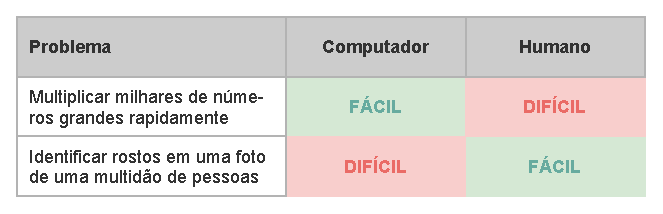
\includegraphics[scale=1.1]{img/img-fundamentacao-dificuldades.pdf}
  \label{fig:fund-dificuldades}
  \indentedfont[15.2cm]{Adaptado de \citeonline{ref:Rashid}}
\end{figure}

A Inteligência Artificial engloba a área de estudo do Aprendizado de Máquina, que por sua vez englobam as áreas do Aprendizado de Representação e Aprendizado Profundo, conforme o diagrama de Venn apresentado na \autoref{fig:fund-ia}.

\begin{figure}[h!] %H
  \centering
  \caption{Diagrama de Venn da Inteligência Artificial e suas áreas de estudo. }
  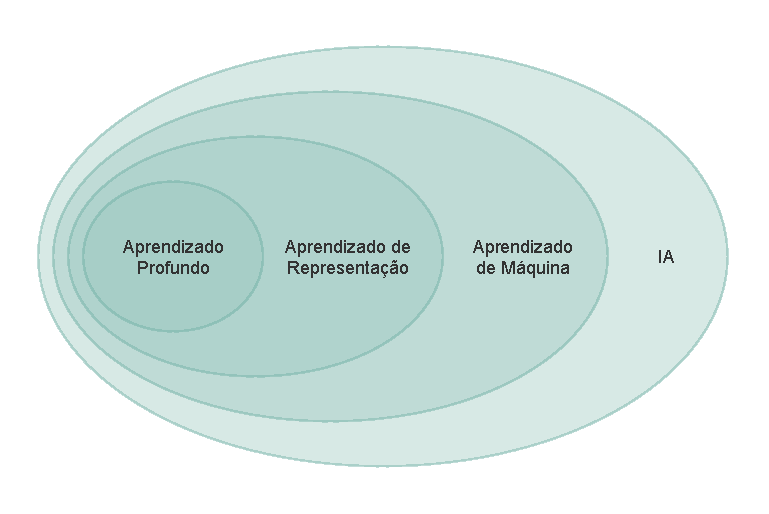
\includegraphics[scale=1.1]{img/img-fundamentacao-ia.pdf}
  \label{fig:fund-ia}
  \indentedfont[15.2cm]{Adaptado de \citeonline{ref:Goodfellow-Bengio-Courville}}
\end{figure}

Para evidenciar as diferenças entre essas áreas de estudo, em comparação com simples Sistemas Baseados em Regras, \citeonline{ref:Goodfellow-Bengio-Courville} apresenta um fluxograma com as etapas de processamento entre a entrada e a saída de dados para cada uma delas, presente na \autoref{fig:fund-fluxograma}.

\begin{figure}[h!] %H
  \centering
  \caption{Fluxograma que diferencia as áreas de estudo da Inteligência Artificial e suas etapas de processamento de dados. }
  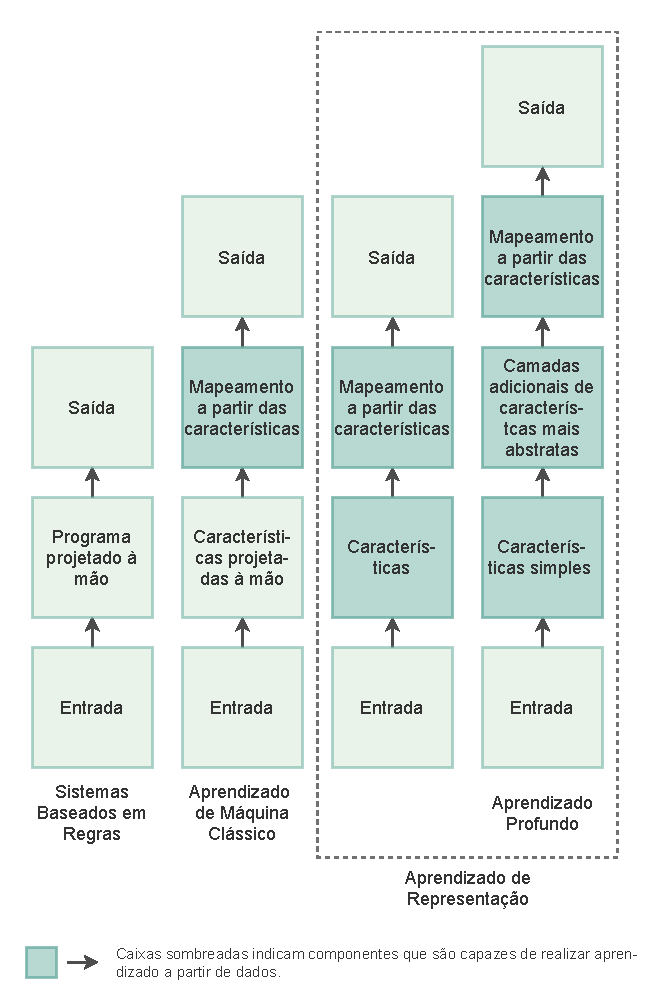
\includegraphics[scale=1.1]{img/img-fundamentacao-fluxograma.pdf}
  \label{fig:fund-fluxograma}
  \indentedfont[15.2cm]{Adaptado de \citeonline{ref:Goodfellow-Bengio-Courville}}
\end{figure}

Sistemas Baseados em Regras não possuem componentes capazes de realizar qualquer aprendizado a partir e dados \cite{ref:Goodfellow-Bengio-Courville} e são utilizados para resolução de problemas e/ou execução de tarefas que podem ser descritos por uma lista de regras formais, como por exemplo jogar Xadrez. Ao contrários desses sistemas, o Aprendizado de Máquina (do inglês \textit{Machine Learning}) utiliza algoritmos computacionais para transformar características reunidas empiricamente em modelos utilizáveis \cite{ref:Edgar-Manz} possuindo a capacidade ``de se aprimorar [...], aprendendo novos conhecimentos ao invés de serem programado com eles'' \cite{ref:Woolf}.

No Aprendizado de Representação (do inglês \textit{Feature Learning} ou \textit{Representation Learning}) entretanto, não há necessidade de mapear manualmente essas características \cite{ref:Goodfellow-Bengio-Courville}. Ou seja, por conta própria e de forma abstrata, os algoritmos são capazes de extrair as características importantes para a construção dos modelos utilizando redes neurais \cite{ref:Robins} \cite{ref:Lesort}. O Aprendizado Profundo, por sua vez, resolve a dificuldade que o Aprendizado de Representação possui de extrair características abstratas de alto nível, tais como sotaques de um locutor \cite{ref:Goodfellow-Bengio-Courville}. Segundo \citeonline{ref:Mao-Wang-Tang-Qian}, o Aprendizado Profundo ``imita a função que o cérebro humano possui de interpretar dados usando redes neurais de várias camadas''. Um exemplo dessas variadas camadas é apresentado na \autoref{fig:fund-camadas}, onde características distintas são extraídas por cada camada. Uma comparação com o modelo de Aprendizado de Máquina é ilustrado na \autoref{fig:fund-aprendizados}.

\begin{figure}[h!] %H
  \centering
  \caption{Ilustração das camadas de um modelo de Aprendizado Profundo.}
  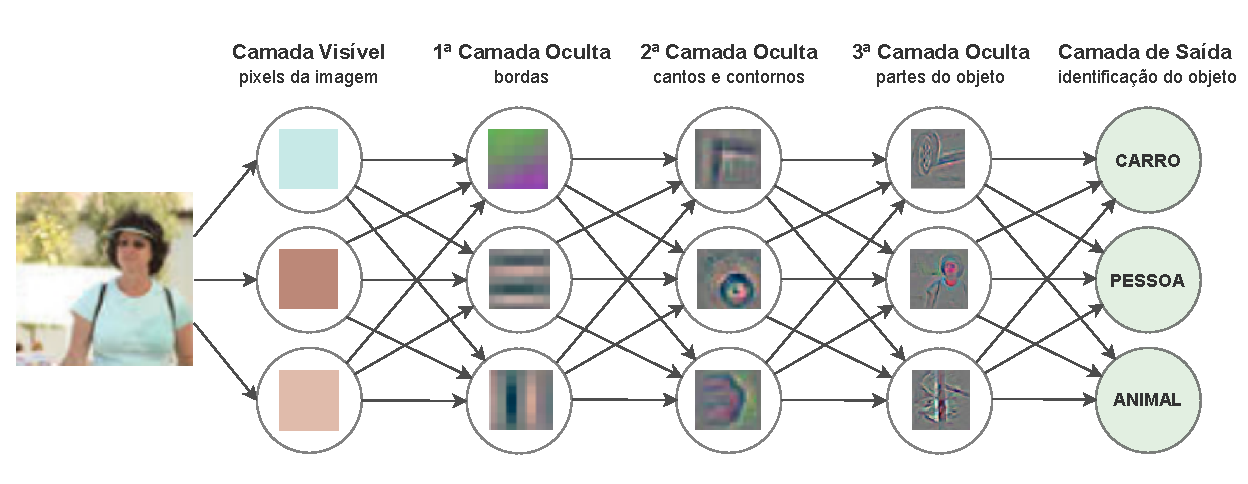
\includegraphics[scale=0.8]{img/img-fundamentacao-deep-learning.pdf}
  \label{fig:fund-camadas}
  \indentedfont[15.2cm]{Adaptado de \citeonline{ref:Goodfellow-Bengio-Courville}}
\end{figure}

\begin{figure}[h!] %H
  \centering
  \caption{Comparação entre os modelos Aprendizado de Máquina e Aprendizado Profundo.}
  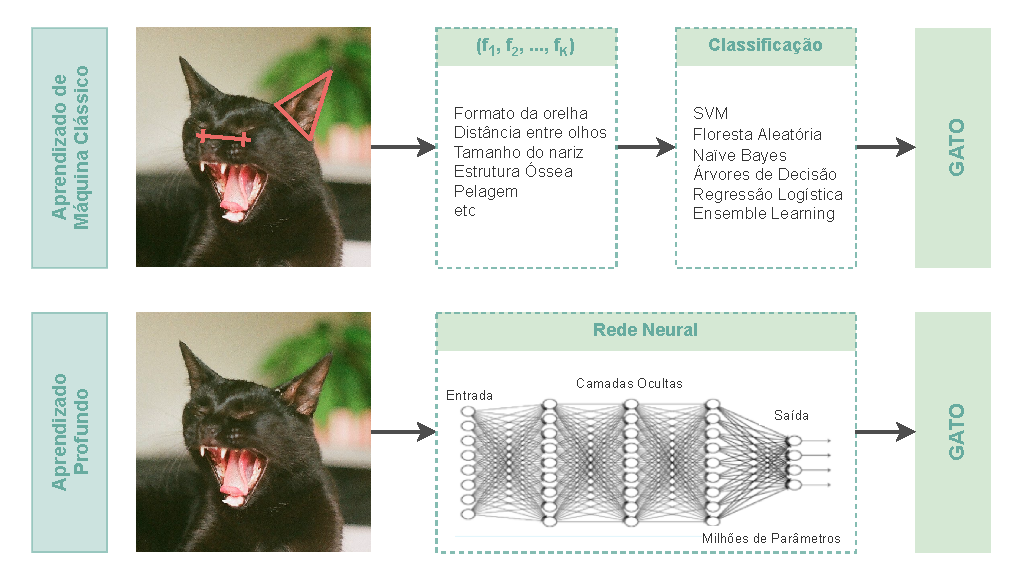
\includegraphics[scale=0.95]{img/img-fundamentacao-aprendizados.pdf}
  \label{fig:fund-aprendizados}
  \indentedfont[15.2cm]{Adaptado de \citeonline{ref:Robins}}
\end{figure}


%%%%%%%%%%%%%%%%%%%%%%%%%%%%%%%%%%%%%%%%%%%%%%%%%%%%%%%%%%%%%%%%%%%%%55
\section{Redes Neurais} \label{cap:fund-ia-rn}
Ao contrário da abordagem convencional de programação, onde dizemos a um computador o que deve ser feito ao dividir um problema em pequenas tarefas para que ele execute, uma Rede Neural (do inglês \textit{Neural Network}) utiliza dados observacionais para aprender como resolver o problema \cite{ref:Nielsen}.

\citeonline{ref:Walczak-Cerpa} define Redes Neurais Artificiais como modelos que ``simulam a atividade elétrica do cérebro e do sistema nervoso''. Porém enquanto alguns tipos de redes neurais tem sido utilizadas para entender o funcionamento do cérebro, na perspectiva de Aprendizado Profundo elas não são projetadas para serem modelos realistas da função biológica \cite{ref:Goodfellow-Bengio-Courville}.

\subsection{Estrutura de Uma Rede Neural} \label{cap:fund-ia-rn-estrutura}
Uma Rede Neural é composta por camadas de nós, conhecidos como neurônios, e conexões que interligam as saídas e entradas desses nós. A estrutura básica de uma Rede Neural é ilustrada na \autoref{fig:fund-nn}, onde a primeira camada de neurônios é a camada de entrada, a última camada é a camada de saída e as camadas entre elas são chamadas de camadas ocultas. Na \autoref{fig:fund-nn}, vetor $\mathrm{X}$ contém os valores de entrada, os vetores $\mathrm{a^{[l]}}$ representam as funções de ativação referentes à \textit{l-ésima} camada, e $\mathrm{\hat{y}}$ é o vetor de saída com os valores preditos. As notações utilizadas nesse capítulo respeitam as propostas por \citeonline{ref:Ng} presentes no \autoref{apendice:notacao}.

\begin{figure}[h!] %H
  \centering
  \caption{Estrutura básica de uma Rede Neural com duas camadas.}
  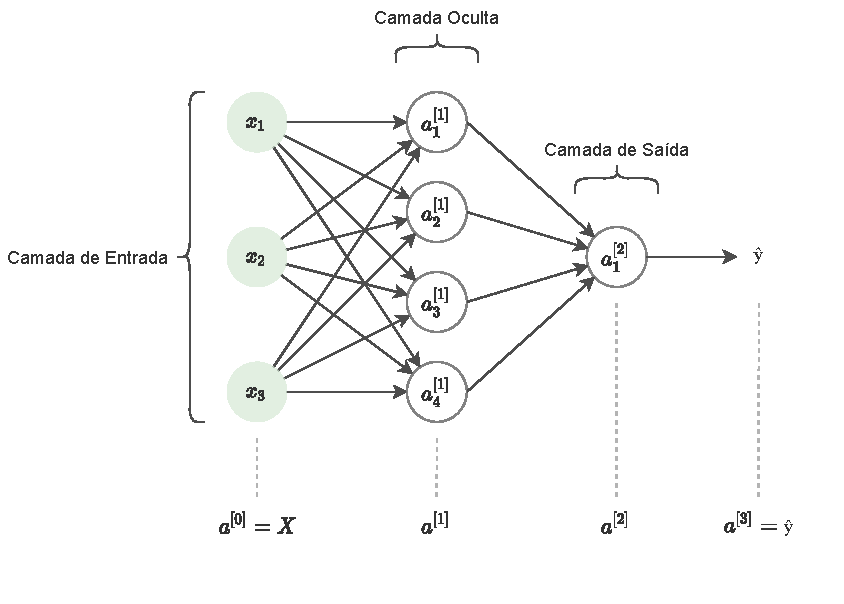
\includegraphics[scale=1.1]{img/img-fundamentacao-nn.pdf}
  \label{fig:fund-nn}
  \indentedfont[15.2cm]{Elaboração própria (2021)}
\end{figure}

São nos neurônios que ocorrem as computações. A \autoref{fig:fund-no} mostra um diagrama de um nó de uma Rede Neural, onde os pesos representados por b e $\mathrm{w_k}$ são responsáveis por atribuir significância às entradas com relação à tarefa que o algoritmo está tentando aprender \cite{ref:Nicholson}. Esses produtos são então somados e passam por uma função de ativação.

\begin{figure}[h!] %H
  \centering
  \caption{Diagrama de um Neurônio de uma Rede Neural.}
  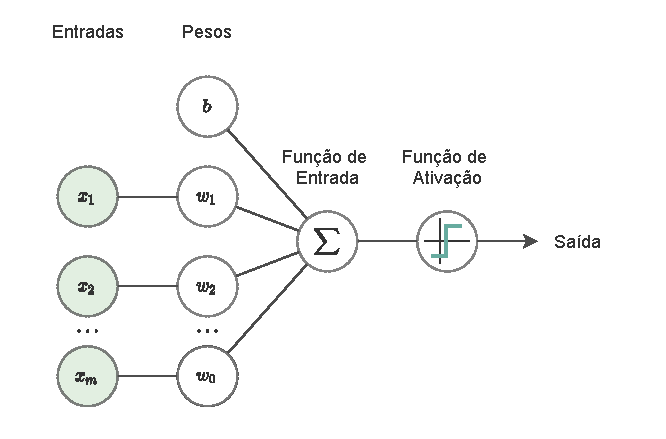
\includegraphics[scale=1.1]{img/img-fundamentacao-no.pdf}
  \label{fig:fund-no}
  \indentedfont[15.2cm]{Adaptado de \citeonline{ref:Nicholson}}
\end{figure}

\subsection{Funções de Ativação} \label{cap:fund-ia-rn-func}
As funções de ativação desempenham um papel crucial na dinâmica de desempenho e treinamento em redes neurais \cite{ref:Misra}, determinando se um sinal deve progredir e em que medida ele deve progredir através da rede \cite{ref:Nicholson}. Alguns exemplos de função de ativação estão na \autoref{fig:fund-funcs}.

\begin{figure}[h!]
    \centering
    \caption{Exemplos de funções de ativação de um neurônio para uma Rede Neural.}
    \begin{subfigure}[H]{.4\textwidth}
        \centering
        \caption{Sigmóide}
        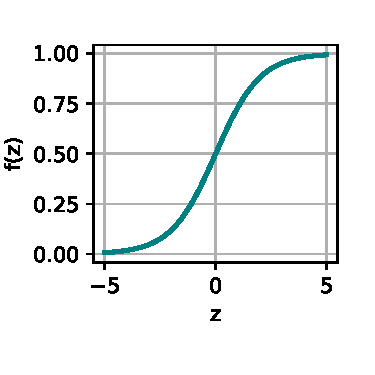
\includegraphics[scale=0.8]{img/img-fundamentacao-sig.pdf}
        \label{fig:fund-funcs-sig}
    \end{subfigure}
    \begin{subfigure}[H]{.4\textwidth}
        \centering
        \caption{Tangente Hiperbólica}
        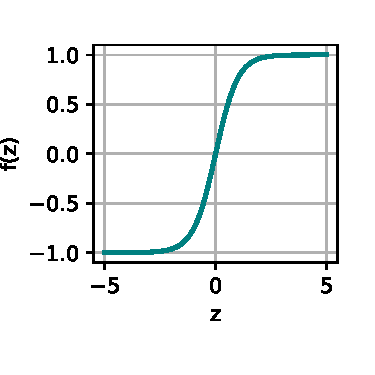
\includegraphics[scale=0.8]{img/img-fundamentacao-tanh.pdf}
        \label{fig:fund-funcs-tanh}
    \end{subfigure}
    \begin{subfigure}[H]{.4\textwidth}
        \centering
        \caption{ReLU}
        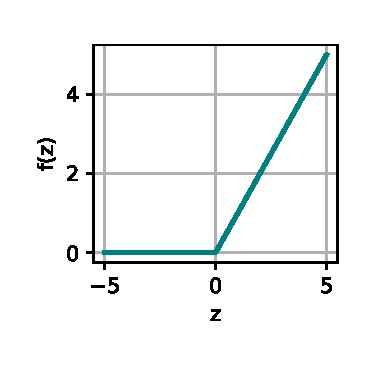
\includegraphics[scale=0.8]{img/img-fundamentacao-relu.pdf}
        %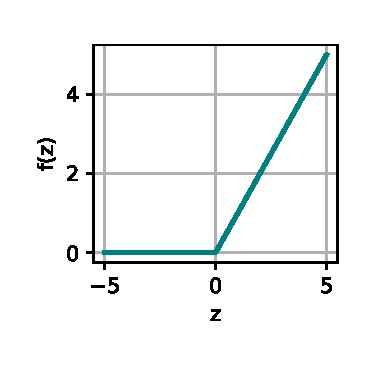
\includegraphics[width=\textwidth]{img/img-fundamentacao-relu.pdf}
        \label{fig:fund-funcs-relu}
    \end{subfigure}
    \begin{subfigure}[H]{.4\textwidth}
        \centering
        \caption{Mish}
        %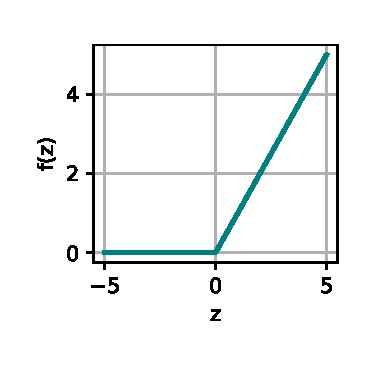
\includegraphics[scale=0.8]{img/img-fundamentacao-relu.pdf}
        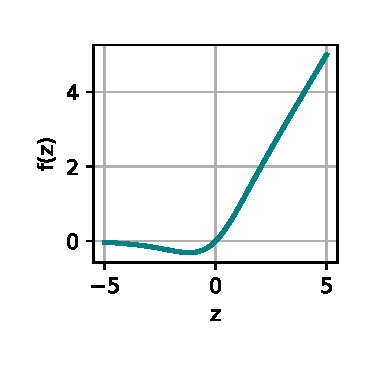
\includegraphics[scale=0.8]{img/img-fundamentacao-mish.pdf}
        \label{fig:fund-funcs-mish}
    \end{subfigure}
    \indentedfont[15.5cm]{Elaboração própria (2021)}
	\label{fig:fund-funcs}
\end{figure}

A função Sigmoide definida pela \autoref{eq:fund-sig} \citeonline{ref:Sharma}  é geralmente utilizada em classificações binárias, pois o resultado está sempre no intervalo entre zero e um \cite{ref:Ng}. A \autoref{fig:fund-funcs-sig} mostra um gráfico da função Sigmoide.

\begin{equation} \label{eq:fund-sig}
  \text{f(z)} = \sigma(z) = \frac{1}{1 + e^{-z}}
\end{equation}

Para a otimização dos pesos durante o treinamento de uma rede neural, em geral é necessário calcular o gradiente das funções de ativação. Por isso, de acordo com \citeonline{ref:Sharma}, o uso da tangente hiperbólica como função de ativação é preferível pois tem gradientes que não estão restritos a variar em uma certa direção e são mais acentuados quando comparado à sigmoide. A definição da tangente hiperbólica da \autoref{fig:fund-funcs-tanh} está na \autoref{eq:fund-tanh}.

\begin{equation} \label{eq:fund-tanh}
  \text{f(z)} = tanh(z) = \frac{e^{z} - e^{-z}}{e^{z} + e^{-z}}
\end{equation}

Porém, para valores muito grandes ou muito pequenos de $\mathrm{z}$, a derivada resultante, utilizada no gradiente, tende a ser nula tanto para a sigmoide quanto para a tangente hiperbólica \cite{ref:Ng} o que geralmente causa lentidão no treinamento \cite{ref:Misra}. Para que isso não ocorra, utiliza-se a função ReLU, do inglês \textit{Rectified Linear Unit}, mostrada na \autoref{fig:fund-funcs-relu} e definida na \autoref{eq:fund-relu}. A ReLU é a função de ativação mais utilizada \cite{ref:Ng} e é a função padrão recomendada para uso com a maioria das redes neurais \cite{ref:Goodfellow-Bengio-Courville}.

\begin{equation} \label{eq:fund-relu}
  \mathrm{{f(z)} = ReLU(z) = max(0, z)}
\end{equation}

Com a evolução das Redes Neurais na última década, diversas funções de ativação vem sendo propostas com o objetivo de melhorar o desempenho do treinamento. Um exemplo delas é a Mish (\autoref{fig:fund-funcs-mish}), proposta por \citeonline{ref:Misra} cuja função é definida pela \autoref{eq:fund-mish}.

\begin{equation} \label{eq:fund-mish}
  \mathrm{{f(z)} = z \cdot tanh(ln(1 + e^z))}
\end{equation}

Segundo \citeonline{ref:Misra}, ao contrário da ReLU, a função Mish é continuamente diferenciável, evitando efeitos colaterais indesejados quando utiliza-se a otimização baseada no método do gradiente.

%\subsection{Conjunto de Dados} \label{cap:treinamento-dataset}

%Utiliza-se para o treinamento da Rede Neural um conjunto de dados, conhecido no inglês como \textit{Dataset}. Geralmente, o conjunto de testes é dividido em três conjuntos menores: Treinamento, utilizado para o treinamento da rede neural; Teste, que é utilizado para saber até quando deve-se prosseguir com o treinamento; e o Conjunto de Validação, que é independente dos outros dois conjuntos \cite{ref:Crowther}.

\subsection{Treinamento de Uma Rede Neural}\label{cap:fund-ia-rn-treinamento}

Para o treinamento de uma Rede Neural, utiliza-se um conjunto de exemplos de treinamento $\{(x^{(1)}, y^{(1)}), \cdots, (x^{(m)}, y^{(m)})\}$, onde $x^{(i)}, y^{(i)}$ são, respectivamente, a entrada e a saída real do \textit{i-ésimo} exemplo de treinamento de um conjunto contendo m exemplos de treinamento \cite{ref:Ng}. Para cada um desses exemplos, o objetivo é fazer o cálculo dos pesos w e b de forma que a saída estimada $\hat{y}^{(i)}$ seja próxima da saída real $y^{(i)}$.

O peso b é chamado de \textit{bias} e não é multiplicado a nenhum valor da entrada para caso todos os valores de x sejam nulos, a saída $\hat{y}^{(i)}$ seja diferente de zero. O cálculo desses pesos é feito de forma iterativa e geralmente são iniciados de forma aleatória.

O processo de cálculo considerando um nó de uma rede neural está ilustrado na \autoref{fig:fund-etapas}, onde a função de ativação utilizada é a sigmoide e todos os valores calculados e os de entrada são representados na forma vetorial.

\begin{figure}[h!] %H
  \centering
  \caption{Estapas da atualização dos pesos de um nó em uma Rede Neural.}
  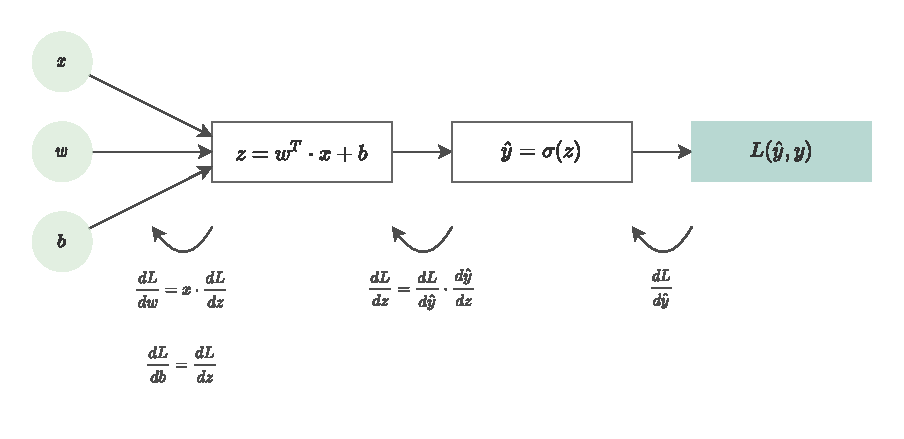
\includegraphics[scale=1.1]{img/img-fundamentacao-etapas.pdf}
  \label{fig:fund-etapas}
  \indentedfont[15.2cm]{Adaptado de \citeonline{ref:Ng}}
\end{figure}

A primeira etapa a ser computada após a passagem das entradas pela função de ativação é função de perda, que mede quão boa é a saída prevista $\hat{y}$ em comparação aos valores verdadeiros de y para apenas um conjunto de treinamento \cite{ref:Ng}.

Um exemplo de função de perda que compara $\mathrm{\hat{y}}$ com y pode ser definida pela \autoref{eq:fund-perda} \cite{ref:Ng}, onde o objetivo do treinamento é obter $L(y,\hat{y}) = 0$.

\begin{equation} \label{eq:fund-perda}
  \mathrm{
    L(y,\hat{y}) = -(y \cdot log(\hat{y}) + (1 - y) \cdot log(1 - \hat{y}))
  }
\end{equation}

Dessa forma, como $\mathrm{\hat{y} = f(w, b)}$, é necessário encontrar valores para os pesos w e b que minimizem a função de perda $L(y,\hat{y})$. Para isso, utiliza-se o método do gradiente, um algoritmo de primeira ordem iterativo utilizado em otimização para encontrar o mínimo local de uma função \cite{ref:Yan}, exemplificado na \autoref{fig:fund-gradiente} para uma função de perda considerando apenas a variável w.

\begin{figure}[h!] %H
  \centering
  \caption{Método do gradiente para uma variável.}
  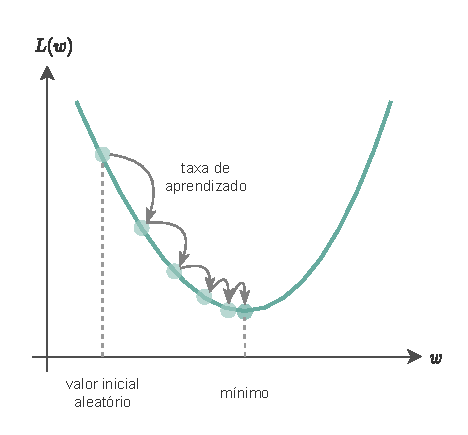
\includegraphics[scale=1.3]{img/img-fundamentacao-gradiente.pdf}
  \label{fig:fund-gradiente}
  \indentedfont[15.2cm]{Adaptado de \citeonline{ref:Sauer}}
\end{figure}


Após serem computadas as derivadas da \autoref{fig:fund-etapas}, os pesos w e b são atualizados conforme a \autoref{eq:fund-atualizacao-w} e a \autoref{eq:fund-atualizacao-b} onde $\alpha$ representa uma taxa de aprendizado \cite{ref:Ng}.

\begin{equation} \label{eq:fund-atualizacao-w}
  \mathrm{
    w = w - \alpha \cdot \frac{dL}{dw}
  }
\end{equation}

\begin{equation} \label{eq:fund-atualizacao-b}
  \mathrm{
    b = b - \alpha \cdot \frac{dL}{db}
  }
\end{equation}

A atualização desses pesos é feita até que a função de perda resulte valores muito próximos de zero ou quando o erro está dentro de uma faixa aceitável de acordo com a métrica de avaliação utilizada.



\subsection{Métricas de Avaliação} \label{cap:fund-ia-metricas}
Determinar os objetivos de treinamento em uma rede neural em termos de qual métrica de erro será utilizada é uma etapa necessária, já que para a maioria das aplicações é impossível obter erro zero absoluto. \cite{ref:Goodfellow-Bengio-Courville}.

\subsubsection{Matriz de Confusão} \label{cap:fund-ia-metricas-matriz}
A Matriz de Confusão é uma técnica muito popular usada em problemas de classificação binária, representando a contagem dos resultados da predição feitos pela rede neural em comparação com os valores reais \cite{ref:Batarseh-Yang}, na forma de verdadeiros positivos, verdadeiros negativos, falsos positivos e falsos negativos. Um exemplo de matriz de confusão utilizada em classificações binárias está na \autoref{fig:fund-matriz}.

\begin{figure}[h!] %H
  \centering
  \caption{Matriz de Confusão para classificação binária.}
  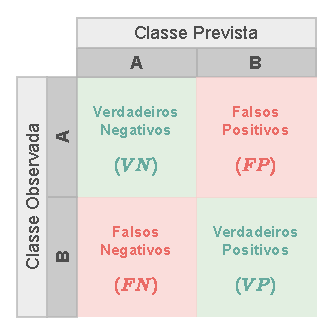
\includegraphics[scale=1.1]{img/img-fundamentacao-matriz.pdf}
  \label{fig:fund-matriz}
  \indentedfont[15.2cm]{Adaptado de \citeonline{ref:Batarseh-Yang}}
\end{figure}

\subsubsection{Acurácia} \label{cap:fund-ia-metricas-acuracia}
Uma das métricas mais comuns utilizadas durante a classificação é a Acurácia \cite{ref:Batarseh-Yang}, que pode ser calculada a partir da matriz de confusão utilizando a \autoref{eq:fund-acuracia}, definida pela razão entre o número de predições corretas e o número total de predições.

\begin{equation} \label{eq:fund-acuracia}
\mathrm{
  Acur\acute{a}cia = \frac{VN + VP}{VN + FP + FN + VP}
}
\end{equation}

A Acurácia pode causar uma impressão incorreta se utilizada como métrica no treinamento de um conjunto de dados desequilibrados, portanto outros métodos baseados na matriz de confusão podem ser utilizados \cite{ref:Batarseh-Yang}, como os métodos de Precisão e Sensibilidade.

\subsubsection{Precisão e Sensibilidade} \label{cap:fund-ia-metricas-pr}

A medida de Precisão (do inglês \textit{Precision}), definida pela \autoref{eq:fund-precisao}, representa a fração de detecções feitas de forma correta; enquanto a Sensibilidade, conhecida do inglês como \textit{Sensitivity} ou \textit{Recall}, representa apenas a fração das predições verdadeiras \cite{ref:Goodfellow-Bengio-Courville}, como mostra a \autoref{eq:fund-sensibilidade}. Ambas métricas fornecem informações importantes a respeito do treinamento, porém o objetivo é melhorar a Sensibilidade sem que a Precisão seja afetada \apud{ref:Chawla}{ref:Batarseh-Yang}. Uma ilustração das medidas de Precisão e Sensibilidade está na \autoref{fig:fund-pr}.

\begin{equation} \label{eq:fund-precisao}
\mathrm{
  Precis\tilde{a}o = \frac{VP}{VP + FP}
}
\end{equation}

\begin{equation} \label{eq:fund-sensibilidade}
\mathrm{
  Sensibilidade = \frac{VP}{VP + FN}
}
\end{equation}

\begin{figure}[h!] %H
  \centering
  \caption{Ilustração das medidas de Precisão e Sensibilidade.}
  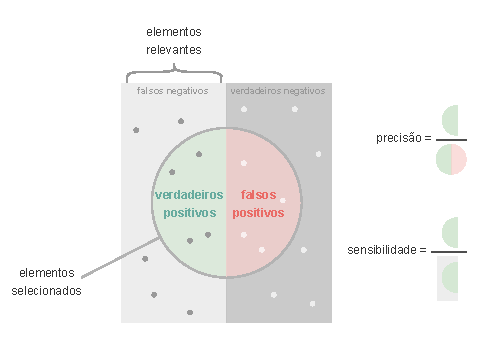
\includegraphics[scale=1.7]{img/img-fundamentacao-pr.pdf}
  \label{fig:fund-pr}
  \indentedfont[15.2cm]{Adaptado de \citeonline{ref:Tan}}
\end{figure}

Uma curva de Precisão em função da Sensibilidade pode ser construída ao variar o \textit{treshold} da probabilidade de um resultado pertencer a determinada classe \cite{ref:Steen}. Um exemplo dessa curva está na \autoref{fig:fund-prcurve}, onde o eixo horizontal indica a Sensibilidade e o eixo vertical, a Precisão para quatro classes distintas.

\begin{figure}[h!] %H
  \centering
  \caption{Curva da Precisão em função da Sensibilidade para quatro classes distintas.}
  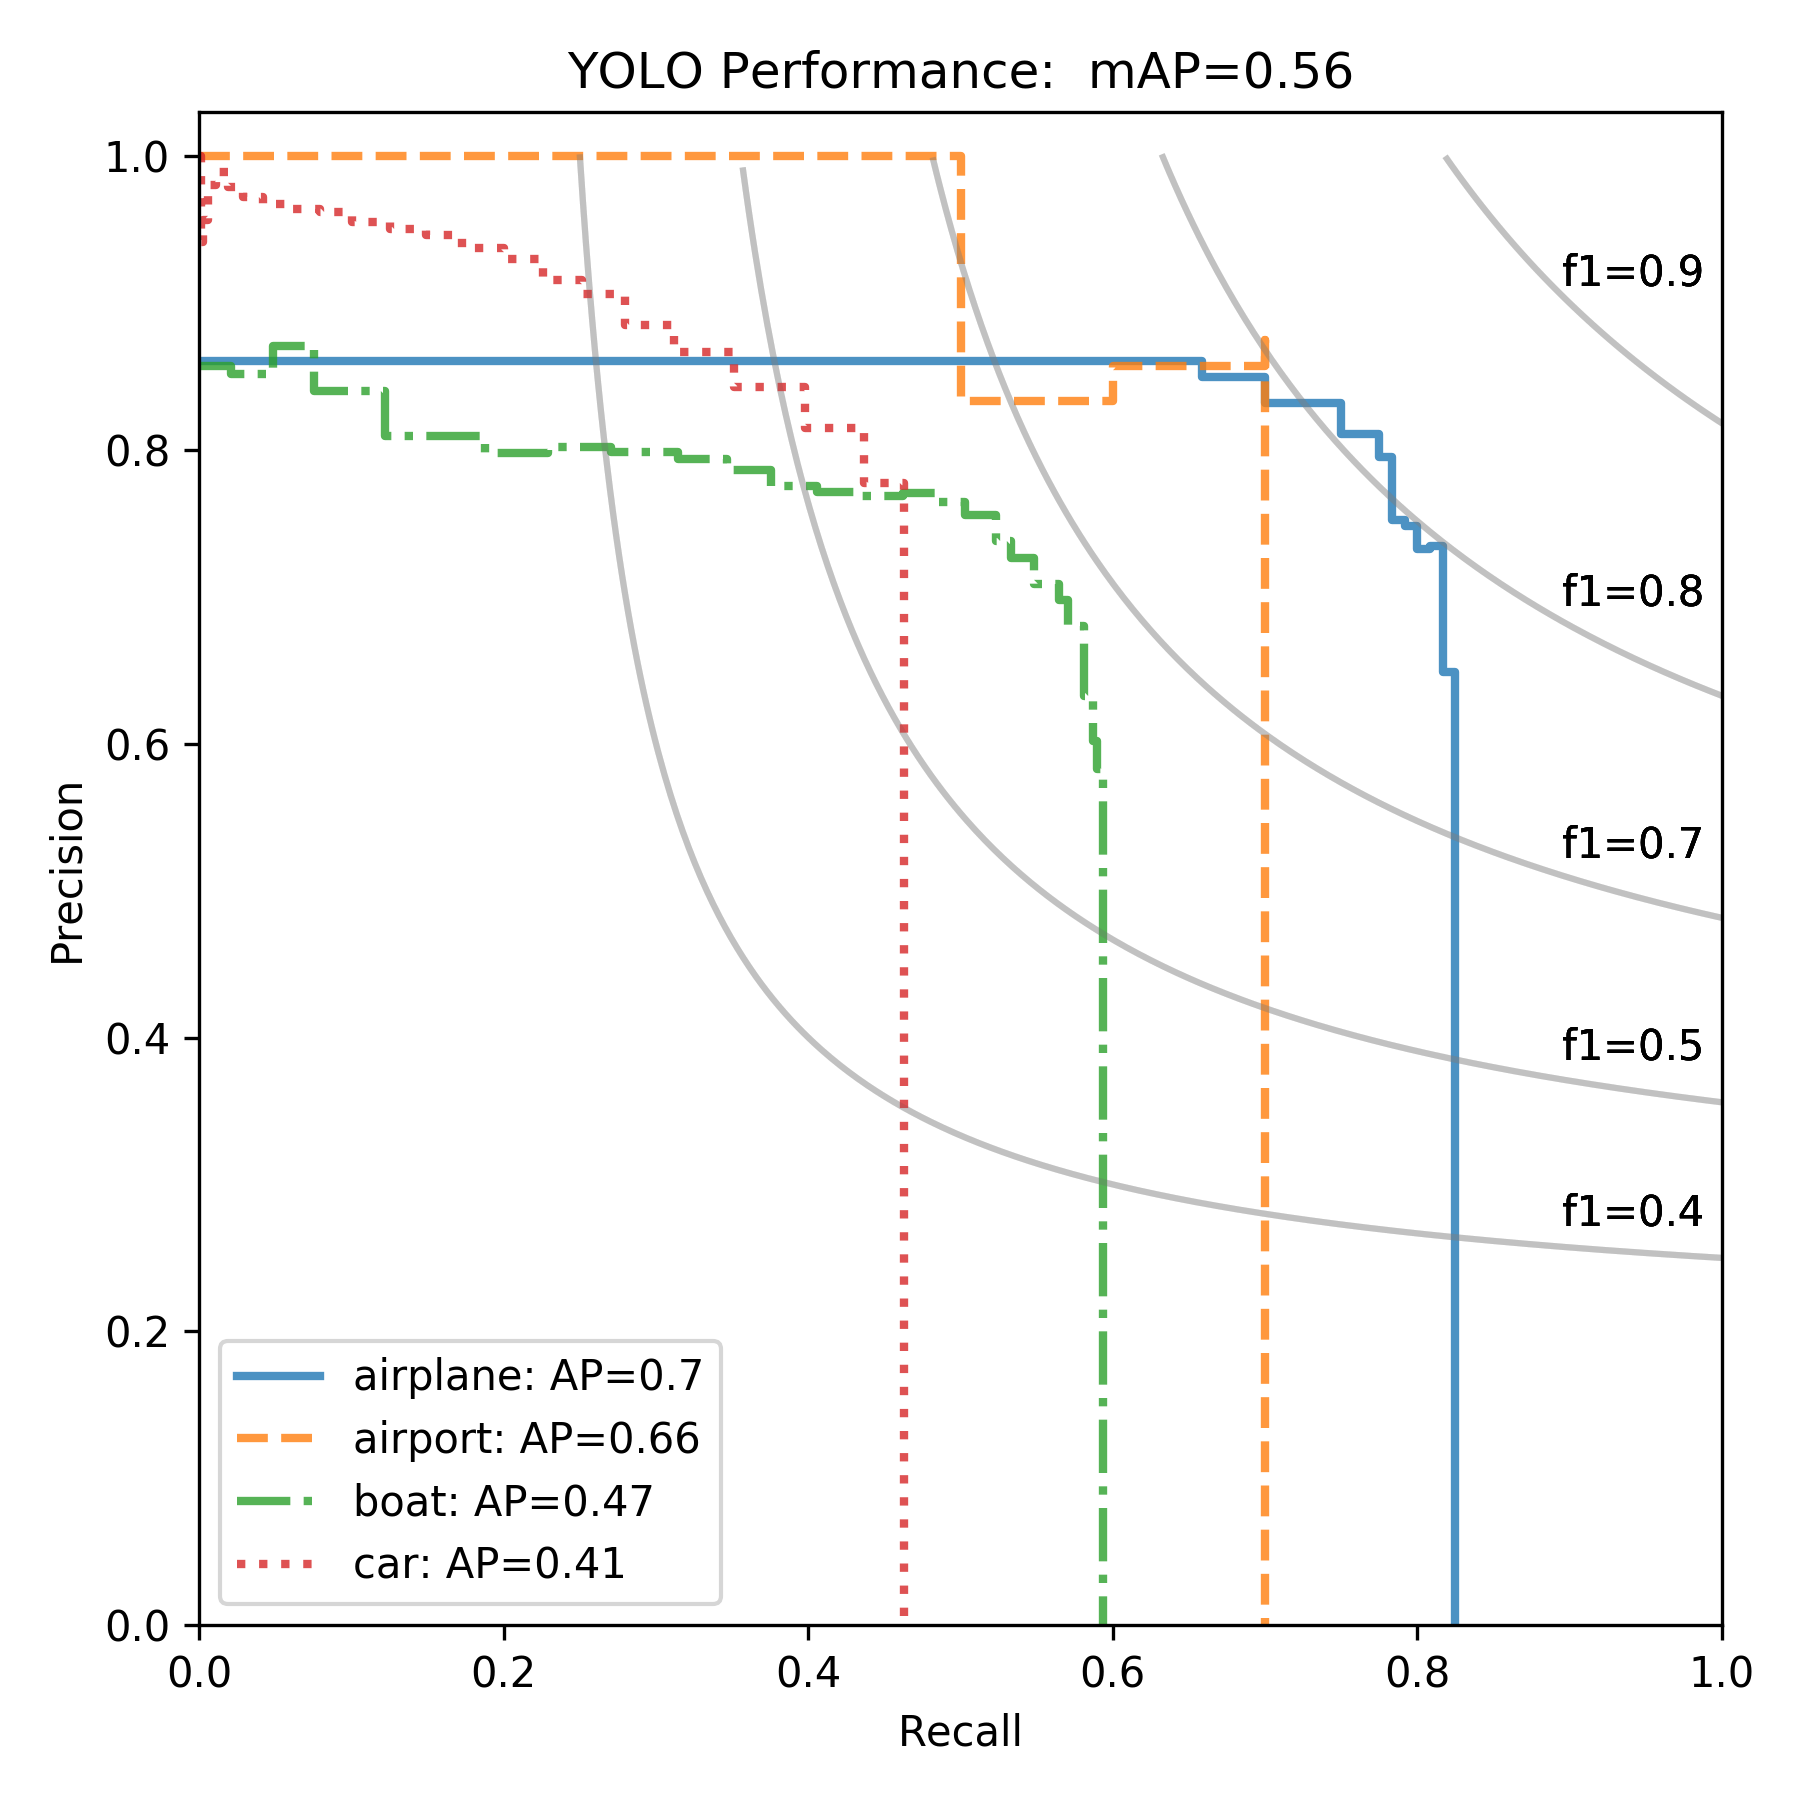
\includegraphics[scale=0.6]{img/img-fundamentacao-prcurve.png}
  \label{fig:fund-prcurve}
  \indentedfont[15.2cm]{\citeonline{ref:Etten}}
\end{figure}

\subsubsection{Precisão Média} \label{cap:fund-ia-metricas-pmed}
O valor da Precisão Média de cada classe, do inglês Average Precision (AP), é encontrado ao calcular a área sob a curva da Precisão em função da Sensibilidade. Já a média desses valores, conhecida no inglês como Mean Average Precision (mAP) é feita como maneira de avaliar um conjunto de treino completo, levando em conta todas as classes treinadas \cite{ref:Tan}.

\subsubsection{\textit{F-Score}} \label{cap:fund-ia-metricas-fscore}
A medida de \textit{F-Score} procura encontrar o equilíbrio entre a Precisão e a Sensibilidade \cite{ref:Mishra} e é feita por meio de uma média harmônica ponderada entre essas medidas \cite{ref:Batarseh-Yang}, conforme a \autoref{eq:fund-fscore}. O resultado está sempre dentro do intervalo entre zero e um e quanto maior o valor de \textit{F-Score}, melhor é a performance do modelo \cite{ref:Mishra}.

\begin{equation} \label{eq:fund-fscore}
\mathrm{
  F-Score = 2 \cdot \frac{Precis\tilde{a}o \cdot Sensibilidade}{Precis\tilde{a}o + Sensibilidade}
}
\end{equation}

\subsubsection{Intersecção sobre União} \label{cap:fund-ia-metricas-iou}
Para avaliar o treinamento da rede neural para detecção de objetos e encontrar os valores das métricas baseadas na matriz de confusão, utiliza-se o conceito de Intersecção sobre União.

A Intersecção sobre União, do inglês \textit{Intersection over Union} (IoU), também conhecida como índice de Jaccard, é a métrica mais  usada para comparar a similaridade entre duas formas arbitrárias \cite{ref:Rezatofighi-et-al}. De forma geral, o IoU pode ser calculado pela \autoref{eq:fund-iou} \cite{ref:Rezatofighi-et-al}, onde a área das formas arbitrárias são representadas pelas letras A e B.

\begin{equation} \label{eq:fund-iou}
\mathrm{
  IoU = \frac{|A \cap B|}{|A \cup B|}
}
\end{equation}

No caso da detecção de objetos em imagens, as formas utilizadas são as caixas delimitadoras desenhadas ao redor dos objetos na imagem, de forma que a IoU é calculada por meio da comparação entre a caixa delimitadora detectada pela rede neural e a localização real do objeto, como ilustra a \autoref{fig:fund-iou}.

\begin{figure}[h!] %H
  \centering
  \caption{Exemplo de caixa delimitadora prevista por uma rede neural em comparação com a localização real do objeto para o cálculo da IoU.}
  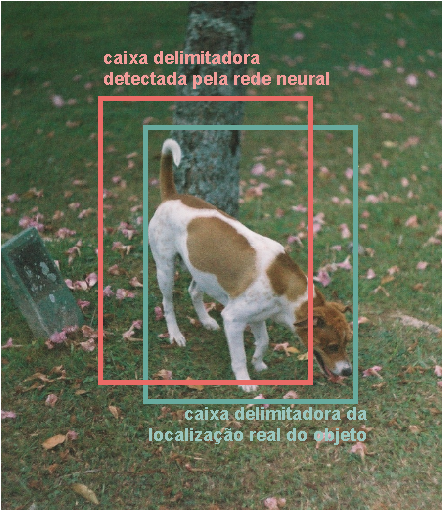
\includegraphics[scale=1.1]{img/img-fundamentacao-iou.pdf}
  \label{fig:fund-iou}
  \indentedfont[15.2cm]{Adaptado de \citeonline{ref:Sivarajkumar}}
\end{figure}



\subsection{Redes Neurais Convolucionais} \label{cap:fund-ia-rn-conv}
Redes Neurais Profundas são caracterizadas por sua grande quantidade de camadas ocultas. Cada uma das camadas é responsável pelo treinamento de um conjunto distinto de dados com base na saída da camada anterior, de forma que quanto mais há avanço pela rede neural, mais complexos são as características que os nós podem reconhecer \cite{ref:Nicholson}, como ilustrado na \autoref{fig:fund-camadas}.

Redes Neurais Convolucionais, do inglês \textit{convolutional neural networks} (CNN), são um tipo de rede neural profunda, originalmente projetadas para análise de imagens \cite{ref:Eden-Ierapetritou-Towler} e tem sido empregadas para esse tipo de processamento desde 1995 \cite{ref:Yan}. O uso de CNNs reduz os requisitos de memória e possui uma melhor eficiência estática quando comparada a redes neurais tradicionais \cite{ref:Goodfellow-Bengio-Courville}.

CNNs sempre contém dois tipos de operações básicas: as operações de convolução e \textit{pooling} \cite{ref:Eden-Ierapetritou-Towler}, além de utilizarem funções de ativação. Os componentes de uma CNN típica estão ilustrados na \autoref{fig:fund-conv}.

\begin{figure}[h!] %H
  \centering
  \caption{Componentes de uma Rede Neural Convolucional típica.}
  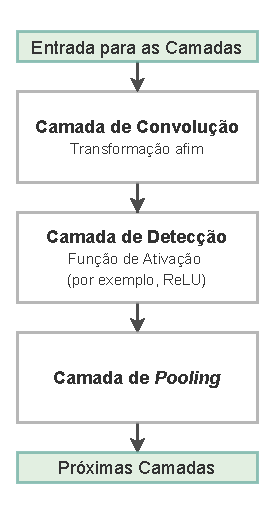
\includegraphics[scale=1.1]{img/img-fundamentacao-conv.pdf}
  \label{fig:fund-conv}
  \indentedfont[15.2cm]{Adaptado de \citeonline{ref:Goodfellow-Bengio-Courville}}
\end{figure}

\subsubsection{Operação de Convolução} \label{cap:fund-ia-rn-conv-conv}

%In convolution layers, CNN uses different kernels for convolving the input image for creating the feature maps

Convolução é uma operação matemática onde duas funções produzem uma terceira função que expressa como o formato de uma é modificado ou filtrado pela outra \cite{ref:Yan}. A operação de convolução em uma rede neural utiliza múltiplos tipos de \textit{kernel} para extrair as características do conjunto de dados da entrada \cite{ref:Eden-Ierapetritou-Towler}, geralmente uma imagem, e cria mapas de características a partir dela \cite{ref:Gholamalinezhad-Khosravi}. O \textit{kernel} usualmente é um vetor de parâmetros multidimensional que é adaptado pelo algoritmo de aprendizado \cite{ref:Goodfellow-Bengio-Courville}, assim como ocorre a atualização dos pesos w e b vistos na \autoref{cap:fund-ia-rn-treinamento}.

Na sua forma discreta, a operação de convolução pode ser definida pela \autoref{eq:fund-conv} \cite{ref:Goodfellow-Bengio-Courville}, onde x representa a entrada e w representa o \textit{kernel} utilizado.

\begin{equation} \label{eq:fund-conv}
\mathrm{
  y[n] = (x \ast w)[n] = \sum_{a = -\infty}^{\infty} x[a] \cdot w [n - a]
}
\end{equation}

Para imagens, as convoluções ocorrem em mais que um eixo ao mesmo tempo. Se a entrada é uma imagem bidimensional I, o \textit{kernel} K provavelmente também será bidimensional, como define a \autoref{eq:fund-conv-2} \cite{ref:Goodfellow-Bengio-Courville}.

\begin{equation} \label{eq:fund-conv-2}
\mathrm{
  Y[i, j] = (I \ast K)[i, j] = \sum_{m} \sum_{n} I[m,n] \cdot K [i-m, j-n]
}
\end{equation}

Porém, utilizando a propriedade comutativa da convolução ao inverter a ordem dos fatores I e K, a implementação se torna mais direta, já que há menos variação no intervalo válido de valores de m e n \cite{ref:Goodfellow-Bengio-Courville}, pois o \textit{kernel} é menor. Além disso, para desinverter o \textit{kernel} em relação à imagem, utiliza-se a operação chamada correlação cruzada \cite{ref:Goodfellow-Bengio-Courville}, como mostra a \autoref{eq:fund-conv-3}.

\begin{equation} \label{eq:fund-conv-3}
\mathrm{
 Y[i, j] = (I \ast K)[i, j] = \sum_{m} \sum_{n} I[i + m,j + n] \cdot K [m,n]
}
\end{equation}

Um exemplo de uma convolução descrita pela \autoref{eq:fund-conv-3} utilizando um \textit{kernel} de 2 x 2 está na figura \autoref{fig:fund-kernel}.

\begin{figure}[h!] %H
  \centering
  \caption{Exemplo de convolução entre dois vetores bidimensionais.}
  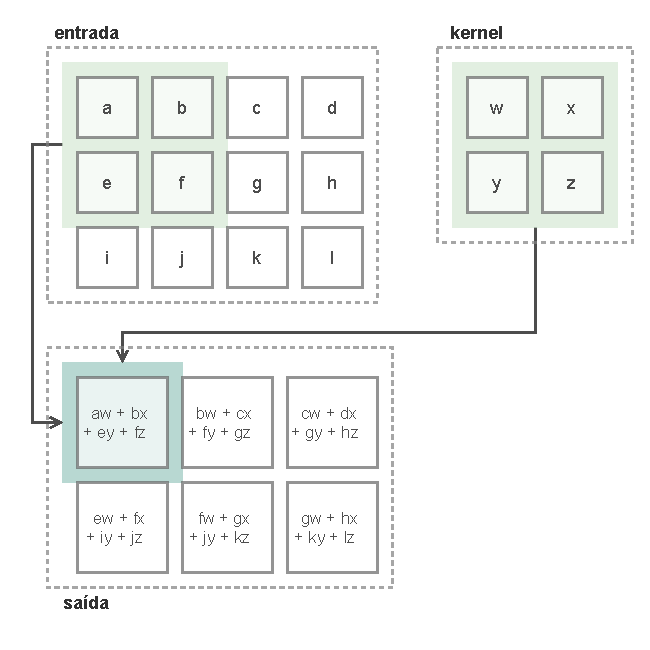
\includegraphics[scale=1.1]{img/img-fundamentacao-kernel.pdf}
  \label{fig:fund-kernel}
  \indentedfont[15.2cm]{Adaptado de \citeonline{ref:Goodfellow-Bengio-Courville}}
\end{figure}

Exemplos de convolução em imagem utilizando distintos tipos de \textit{kernel} está na \autoref{fig:fund-fifits}.

\begin{figure}[h!] %H
  \centering
  \caption{Operações de convolução em uma imagem.}
  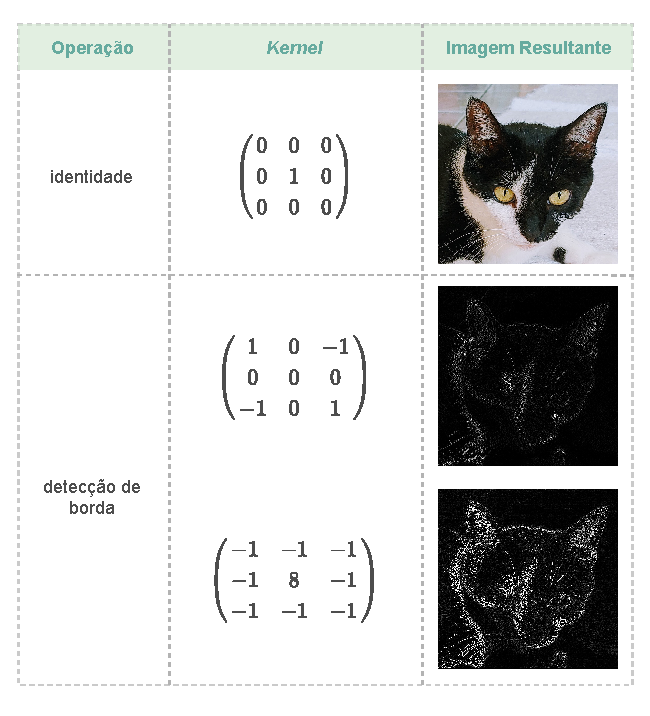
\includegraphics[scale=1.1]{img/img-fundamentacao-fifits.pdf}
  \label{fig:fund-fifits}
  \indentedfont[15.2cm]{Adaptado de \citeonline{ref:Albawi-Mohammed-Al-Zawi}}
\end{figure}

\subsubsection{Operação de \textit{Pooling}} \label{cap:fund-ia-rn-conv-pool}
As operações de \textit{pooling} geralmente são utilizadas após as camadas de convolução para simplificar as informações das saídas dessas camadas \cite{ref:Nielsen} ao reduzir o tamanho do mapa de características \cite{ref:Gholamalinezhad-Khosravi} e ajudam a tornar as saídas aproximadamente invariantes a pequenas modificações da entrada \cite{ref:Goodfellow-Bengio-Courville}.

Espera-se que uma camada de \textit{pooling} ideal extraia somente as informações úteis e descarte detalhes irrelevantes \cite{ref:Gholamalinezhad-Khosravi}. A \autoref{fig:fund-pool} apresenta algumas das funções de \textit{pooling}. A operação de \textit{Max-Pooling} seleciona o pixel com maior valor dentre os píxeis de uma região (\autoref{fig:fund-pool-max}) e a operação de \textit{Pooling} médio (\autoref{fig:fund-pool-av}) faz a média entre esses píxeis.

\begin{figure}[h!]
    \centering
    \caption{Exemplos de funções utilizadas para operação de \textit{pooling}.}
    \begin{subfigure}[H]{.5\textwidth}
        \centering
        \caption{\textit{Pooling} Médio}
        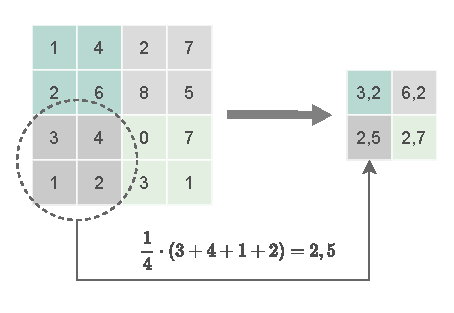
\includegraphics[scale=1.1]{img/img-fundamentacao-av-pool.pdf}
        \label{fig:fund-pool-av}
    \end{subfigure}
    \begin{subfigure}[H]{.5\textwidth}
        \centering
        \caption{\textit{Max-Pooling}}
        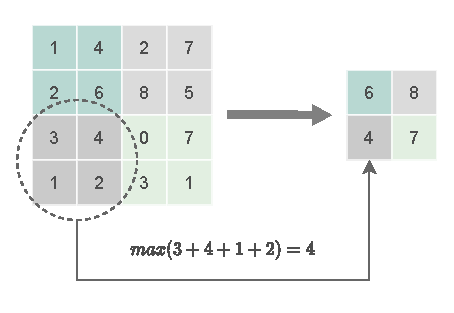
\includegraphics[scale=1.1]{img/img-fundamentacao-max-pool.pdf}
        \label{fig:fund-pool-max}
    \end{subfigure}
    \indentedfont[15.5cm]{Adaptado de \citeonline{ref:Gholamalinezhad-Khosravi}}
	\label{fig:fund-pool}
\end{figure}

\subsubsection{\textit{You Only Look Once}} \label{cap:fund-ia-rn-yolo}
\textit{You Only Look Once} (YOLO), cuja tradução direta do inglês é ``você olha apenas uma vez'', é uma rede neural de passagem única \cite{ref:Yan} onde, ao contrário de outras abordagens, uma única rede neural é aplicada na imagem para fazer a localização e a detecção do objeto, dividindo a imagem em regiões menores e fazendo a previsão e a probabilidade da detecção para cada uma das regiões \cite{ref:Redmon-Farhadi}.

A rede neural YOLO possui 24 camadas convolucionais seguidas por duas camadas totalmente conectadas \cite{ref:Yan}. A arquitetura básica da primeira versão está na \autoref{fig:fund-yoloarq}.

\begin{figure}[h!] %H
  \centering
  \caption{Arquitetura da Rede Neural YOLO.}
  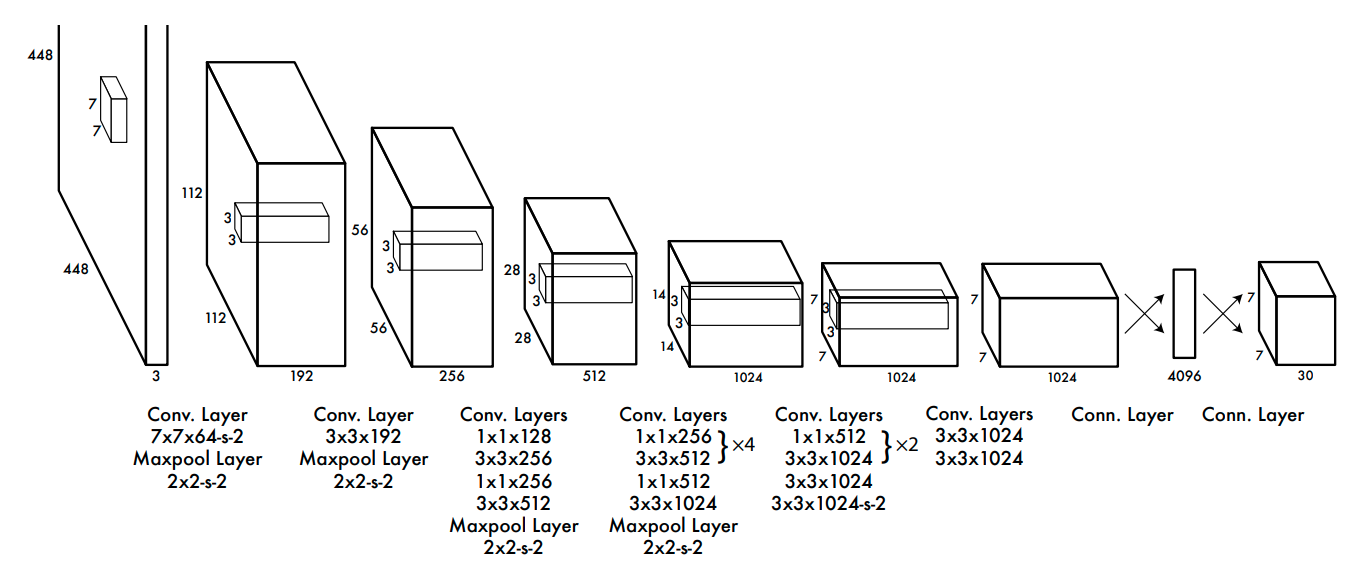
\includegraphics[scale=0.3]{img/img-fundamentacao-yoloarq.png}
  \label{fig:fund-yoloarq}
  \indentedfont[15.2cm]{\citeonline{ref:Redmon-et-al}}
\end{figure}

Atualmente, a rede neural YOLO está na versão 4, apresentando otimização em funções de ativação (utilizando a função Mish da \autoref{fig:fund-funcs-mish} para algumas camadas), processamento dos dados, treinamento, funções de perda, etc, em comparação com a versão anterior \cite{ref:Wang-et-al}.

Uma comparação de desempenho com outras redes neurais utilizadas para detecção de objetos em tempo real está no gráfico da \autoref{fig:fund-yolov4}, que avalia a precisão média em função da quantidade de \textit{frames} por segundo que a rede consegue processar, utilizando o \textit{dataset} \textit{Microsoft COCO:  Common Objects in Context} \cite{ref:Lin-et-al}.

\begin{figure}[h!] %H
  \centering
  \caption{Comparação da precisão média em função do processamento em \textit{frames} por segundo para diferentes redes neurais utilizadas em detecção de objetos.}
  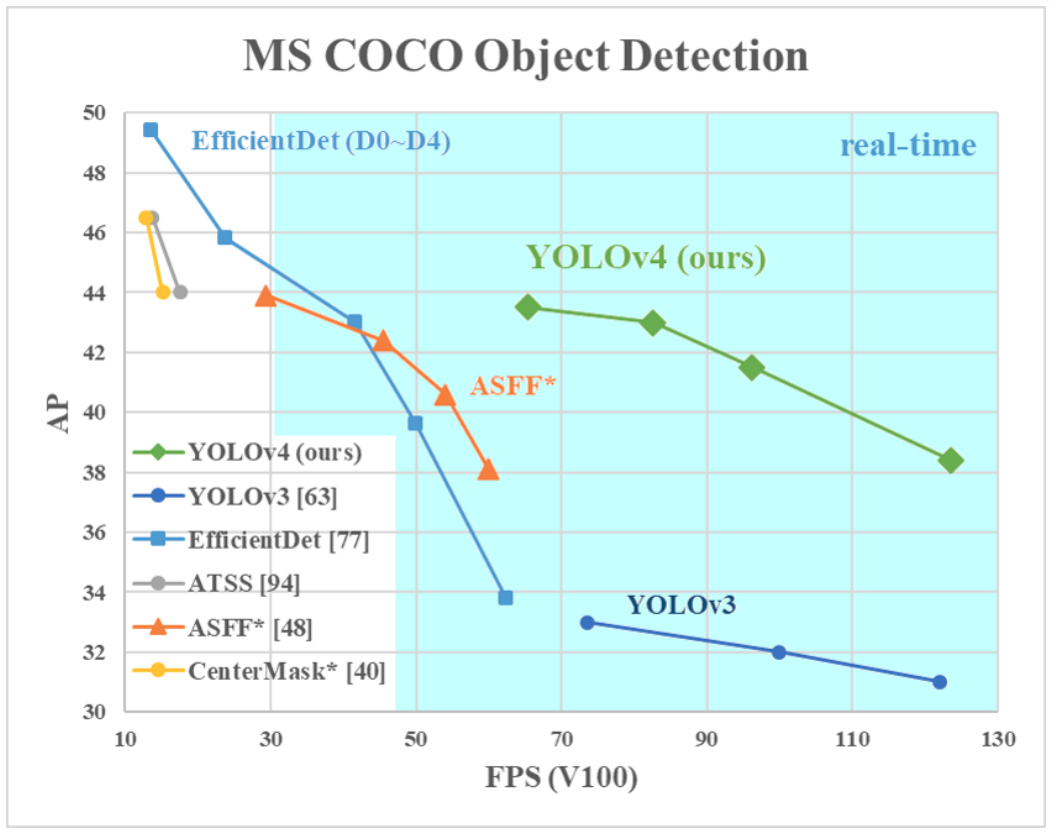
\includegraphics[scale=0.3]{img/img-fundamentacao-yolov4.png}
  \label{fig:fund-yolov4}
  \indentedfont[15.2cm]{\citeonline{ref:Bochkovskiy-Wang-Liao}}
\end{figure}

A YOLO divide a imagem em blocos menores no formato de uma grade, e para cada uma dessas divisões, são previstas caixas delimitadoras, com suas confianças e probabilidades \cite{ref:Redmon-et-al}. A maioria dessas divisões não contém um objeto detectado e a filtragem é feita com base na probabilidade da classe do objeto, onde apenas as caixas delimitadoras de maior probabilidade permanecerão \cite{ref:Sivarajkumar}. Esse processo é ilustrado na \autoref{fig:fund-yolograde}.

\begin{figure}[h!] %H
  \centering
  \caption{Processo de detecção e classificação na rede neural YOLO.}
  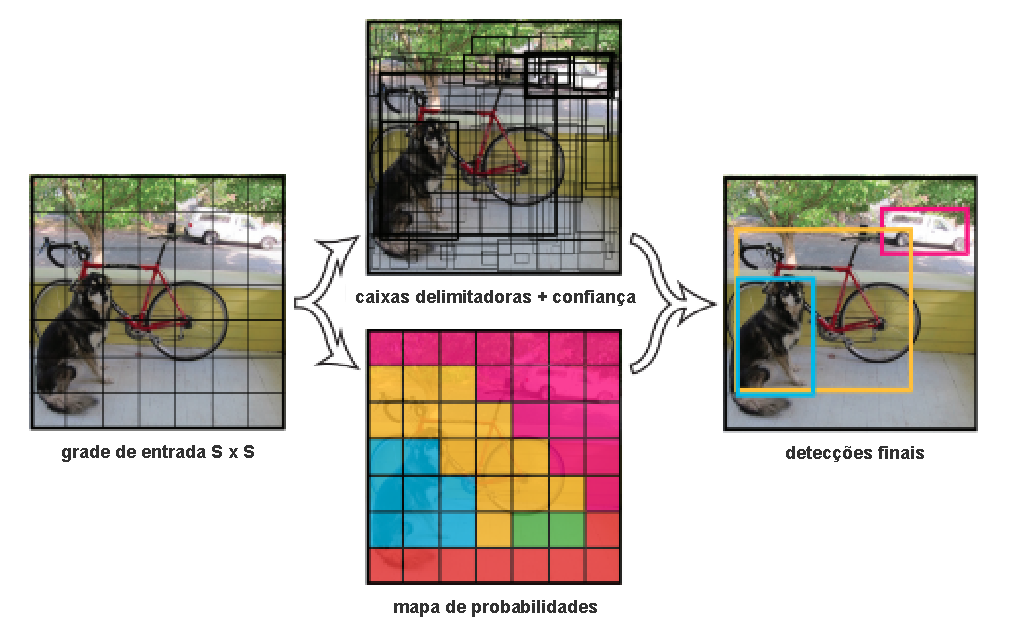
\includegraphics[scale=0.95]{img/img-fundamentacao-yolograde.pdf}
  \label{fig:fund-yolograde}
  \indentedfont[15.2cm]{Adaptado de \citeonline{ref:Redmon-et-al}}
\end{figure}

A camada final é responsável por prever as probabilidades das classes treinadas e as coordenadas das caixas delimitadoras \cite{ref:Redmon-et-al}. Tanto a largura e a altura das caixas delimitadoras quanto as coordenadas x e y são normalizadas pela altura e largura da imagem, de modo que os valores fiquem dentro do intervalo entre zero e um \cite{ref:Redmon-et-al}.

Para o treinamento, são necessárias algumas configurações de arquivos, além da adição das imagens do \textit{dataset} utilizado, a partir do \textit{download} do repositório do projeto disponibilizado por \citeonline{ref:Bochkovskiy}. As instruções a serem seguidas, conforme \citeonline{ref:Bochkovskiy}, estão no \autoref{apendice:etapas-yolo}.

\section{Classificação e Detecção de Defeitos em Placas de Circuito Impresso} \label{cap:fund-pcb}

A classificação e detecção de um objeto em uma imagem são duas tarefas distintas. Segundo \citeonline{ref:Chen-et-al}, ``a tarefa de classificação de objetos visa prever a existência de objetos dentro das imagens, enquanto a tarefa de detecção de objetos visa localizar os objetos'', como mostra a \autoref{fig:fund-deteccaoclassificacao}.

\begin{figure}[h!] %H
  \centering
  \caption{Diferença entre as tarefas de classificação e detetecção de objetos em uma imagem.}
  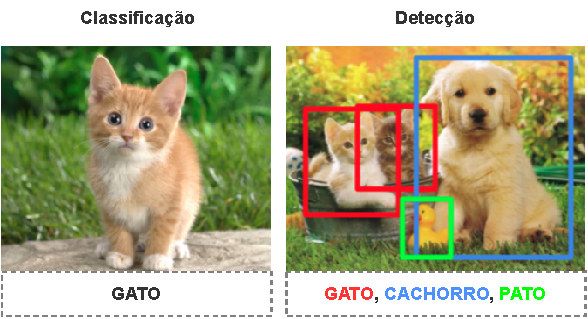
\includegraphics[scale=1.1]{img/img-fundamentacao-deteccaoclassificacao.pdf}
  \label{fig:fund-deteccaoclassificacao}
  \indentedfont[15.2cm]{Adaptado de \citeonline{ref:Sivarajkumar}}
\end{figure}

Considerando Placas de Circuito Impresso (PCIs), os defeitos da etapa de fabricação são localizados e detectados antes da etapa de soldagem dos componentes. Esses defeitos podem ser classificados como circuito aberto, curto-circuito, falta de cobre, cobre excessivo, trilha desconectada e falta de estanho \cite{ref:Ding-et-al}, conforme a \autoref{fig:fund-defeitos}.

\begin{figure}[h!]
    \centering
    \caption{Tipos de defeito de fabricação em placas de circuito impresso.}
    \begin{subfigure}[H]{0.3\textwidth}
        \centering
        \caption{trilha desconectada}
        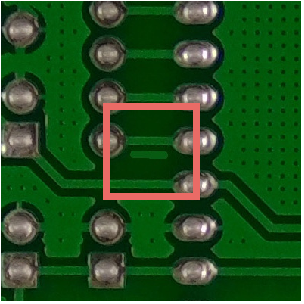
\includegraphics[scale=0.6]{img/img-fundamentacao-defeitos.pdf}
        \label{fig:fund-defeitos1}
    \end{subfigure}
    \begin{subfigure}[H]{0.3\textwidth}
        \centering
        \caption{falta de estanho}
        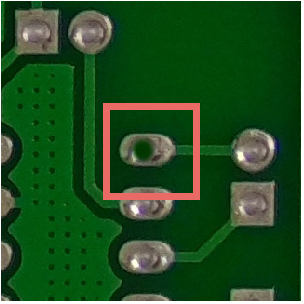
\includegraphics[scale=0.6]{img/img-fundamentacao-defeitos2.pdf}
        \label{fig:fund-defeitos2}
    \end{subfigure}
    \begin{subfigure}[H]{0.3\textwidth}
        \centering
        \caption{falta de cobre}
        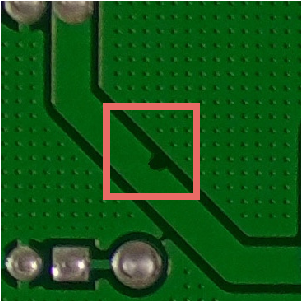
\includegraphics[scale=0.6]{img/img-fundamentacao-defeitos3.pdf}
        \label{fig:fund-defeitos3}
    \end{subfigure}
    \begin{subfigure}[H]{0.3\textwidth}
        \centering
        \caption{excesso de cobre}
        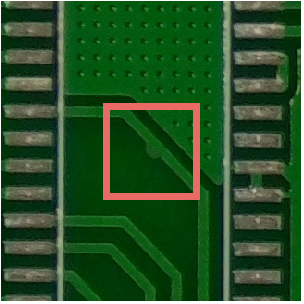
\includegraphics[scale=0.6]{img/img-fundamentacao-defeitos5.pdf}
        \label{fig:fund-defeitos5}
    \end{subfigure}
    \begin{subfigure}[H]{0.3\textwidth}
        \centering
        \caption{curto-circuito}
        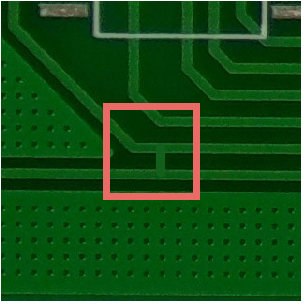
\includegraphics[scale=0.6]{img/img-fundamentacao-defeitos4.pdf}
        \label{fig:fund-defeitos4}
    \end{subfigure}
    \begin{subfigure}[H]{0.3\textwidth}
        \centering
        \caption{circuito aberto}
        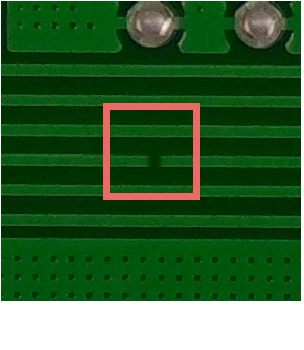
\includegraphics[scale=0.6]{img/img-fundamentacao-defeitos6.pdf}
        \label{fig:fund-defeitos6}
    \end{subfigure}
    \indentedfont[15.5cm]{Adaptado de \citeonline{ref:Huang-et-al}}
	\label{fig:fund-defeitos}
\end{figure}

\subsection{Métodos Automatizados de Extração de Defeitos} \label{cap:fund-pcb-metodos}

Assim como os componentes eletrônicos utilizados em PCIs estão ficando cada vez menores, as placas de circuito impresso também estão diminuindo e se tornando mais delicadas e sofisticadas \cite{ref:Hu-Wang}. Dessa forma, utilizar técnicas automatizadas para detecção e classificação dos defeitos em PCIs é indispensável, já que a inspeção humana além de imprecisa, está associada também à subjetividade, fadiga, lentidão e alto custo \cite{ref:Leta-Feliciano-Martins}.

Diversos métodos de detecção e classificação de defeitos em PCIs vem sendo utilizados nas últimas décadas, podendo ser classificados como métodos comparativos, não-referenciais e híbridos \apud{ref:Moganti-et-al}{ref:Ding-et-al}.

\subsubsection{Métodos Comparativos} \label{cap:fund-pcb-metodos-comp}
Os métodos comparativos de detecção, também conhecidos como métodos referenciais, utilizam uma imagem de referência para extrair os objetos da imagem a ser testada.

Uma das formas de fazer a extração dos defeitos é utilizando a operação lógica de ou-exclusivo (XOR) entre as duas imagens binarizadas, de forma que se o pixel da imagem a ser testada corresponde com o pixel da imagem de referência, o resultado será um, do contrário, o resultado será zero \cite{ref:Huang-et-al}.

A grande dificuldade da operação XOR é determinar o alinhamento preciso entre as duas imagens \cite{ref:Ding-et-al}, além de que ruídos externos podem mascarar os defeitos. \citeonline{ref:Huang-et-al} propõe o uso de algoritmos de registro de imagem para corrigir o desalinhamento entre as imagens. Esses algoritmos extraem as características de ambas imagens, calculando uma matriz de transformação que rotacionará a imagem teste deixando na mesma orientação da imagem de referência \cite{ref:Huang-et-al}. Já para remover os ruídos externos, é proposta por \citeonline{ref:Huang-et-al} a utilização de operações morfológicas, tais como filtros medianos e operações morfológicas de fechamento e abertura. Essas operações são feitas após a operação de XOR, e uma comparação entre o resultado antes e depois das operações morfológicas está na \autoref{fig:fund-morf}.

\begin{figure}[h!]
    \centering
    \caption{Extração de defeitos em placas de circuito impresso utilizando métodos comparativos.}
    \begin{subfigure}[H]{0.8\textwidth}
        \centering
        \caption{resultados após a operação de ou-exclusivo}
        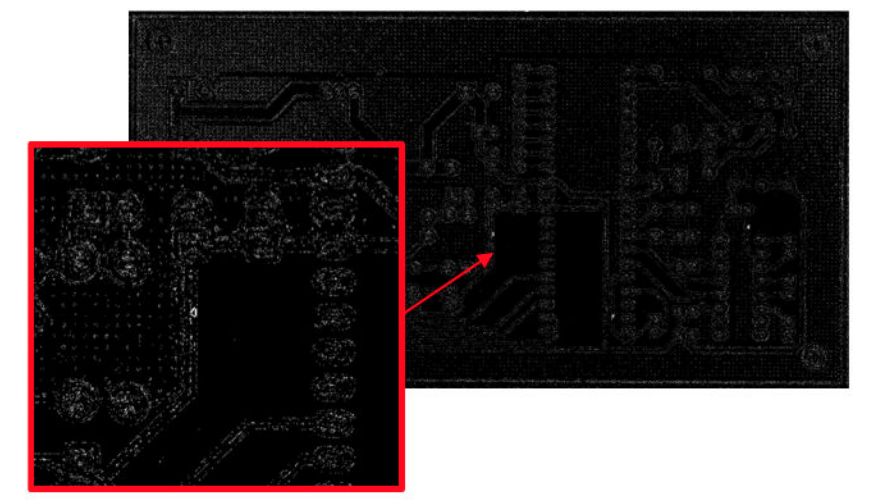
\includegraphics[scale=0.35]{img/img-fundamentacao-morf-xor.png}
        \label{fig:fund-morf-1}
    \end{subfigure}
    \begin{subfigure}[H]{0.8\textwidth}
        \centering
        \caption{resultado após operações morfológicas}
        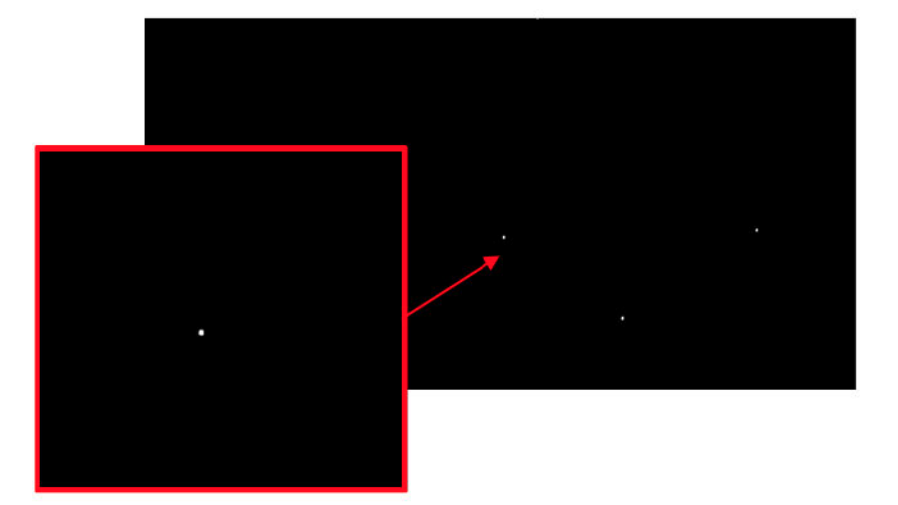
\includegraphics[scale=0.35]{img/img-fundamentacao-morf-morf.png}
        \label{fig:fund-morf-2}
    \end{subfigure}
    \indentedfont[15.5cm]{\citeonline{ref:Huang-et-al}}
	\label{fig:fund-morf}
\end{figure}

No entanto, de acordo com \citeonline{ref:Ding-et-al}, obter uma imagem de referência totalmente sem defeitos em um ambiente de produção é considerado fora da realidade, além de que problemas críticos de desalinhamento, variação de cor, variação de luz, e outras variações, tornam essa tarefa ainda mais custosa.

\subsubsection{Métodos Não-Referenciais} \label{cap:fund-pcb-metodos-nref}
De acordo com \citeonline{ref:Ding-et-al}, os métodos não-referenciais para detecção e classificação de defeitos são baseados na verificação de regras gerais de projeto e, nos últimos anos, o uso de redes neurais profundas tem sido empregadas nessa tarefa. Contudo, conforme \citeonline{ref:Tang-et-al}, usar redes neurais para essa aplicação implica em encontrar um equilíbrio entre eficiência e a alta precisão, já que detecções mais precisas requerem modelos de redes neurais mais profundas para obter características de mais alto nível e detecções mais eficientes precisam de modelos menos profundos para processamentos mais rápidos.

\subsubsection{Métodos Híbridos} \label{cap:fund-pcb-metodos-hib}
Os métodos híbridos combinam os métodos comparativo e não-referencial para a detecção e classificação de defeitos. Um exemplo para a aplicação de detecção e classificação de defeitos é a abordagem RBCNN proposta por \citeonline{ref:Huang-et-al}, onde os defeitos são inicialmente localizados utilizando métodos comparativos e, posteriormente, redes neurais convolucionais são utilizadas para a classificação, conforme o fluxograma da \autoref{fig:fund-hib}.

\begin{figure}[h!] %H
  \centering
  \caption{Fluxograma das etapas para classificação e detecção de defeitos utilizadas na abordagem híbrida RBCNN.}
  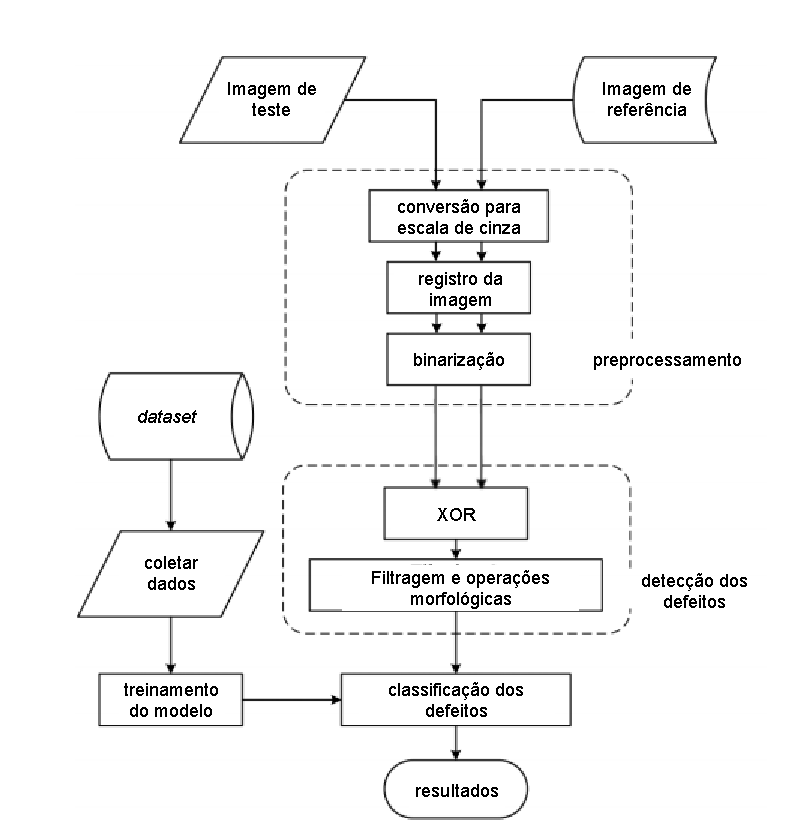
\includegraphics[scale=0.85]{img/img-fundamentacao-hib.pdf}
  \label{fig:fund-hib}
  \indentedfont[15.2cm]{Adaptado de \citeonline{ref:Huang-et-al}}
\end{figure}

%\subsection{\textit{Datasets} Disponíveis} \label{cap:fund-pcb-datasets}

\section{\textit{Frameworks} e Bibliotecas para Detecção e Classificação de Objetos} \label{cap:fund-frameworks}
\textit{Frameworks} e Bibliotecas são códigos utilizados para resolver problemas comuns, evitando a criação de códigos repetidos. Uma biblioteca é responsável por oferecer um conjunto de funcionalidades prontas para o uso, enquanto \textit{frameworks} são um conjunto de bibliotecas que não fornecem apenas funcionalidades, mas também a arquitetura para o desenvolvimento \cite{ref:Tamenaoul}.

%Considerando o contexto de detecção e classificação de objetos utilizando redes neurais, existe uma grande variedades de \textit{frameworks} e bibliotecas que podem ser utilizados, compatíveis com diferentes linguagens de programação.

\subsection{Darknet} \label{cap:fund-frameworks-darknet}
Darknet é um \textit{framework} de código aberto para redes neurais escrito em C e CUDA, com fácil instalação e suporte à computação em CPU e GPU \cite{ref:Redmon}.

\subsection{Flask} \label{cap:fund-frameworks-flask}
Flask é um \textit{framework} para \textit{web} escrito em Python, comumente utilizado por empresas como ferramenta para soluções rápidas e simples \cite{ref:Copperwaite-Leifer}.
Flask também é escalável para desenvolvimento de aplicativos de grande escala \cite{ref:Aggarwal}, fornecendo um conjunto de bibliotecas para lidar com tarefas mais comuns de desenvolvimento \textit{web} \cite{ref:Copperwaite-Leifer}. \citeonline{ref:Copperwaite-Leifer} lista algumas de suas principais funcionalidades:

\begin{itemize}
  \item Roteamento de URLs tornando o mapeamento mais fácil para o código;
  \item Gerenciamento de sessão e proteção de cookies;
  \item Depurador interativo baseado na web;
  \item Gerenciamento de configuração de aplicativo flexível e fácil de usar;
  \item Análise de solicitação HTTP.
\end{itemize}

%\chapter{Metodologia}

Esse trabalho procura encontrar um método de detecção de defeitos de fabricação em placas de circuito impresso, buscando uma solução eficiente e precisa, comparando a solução proposta com outras soluções já testadas. 

%Este trabalho busca apresentar e estudar os possíveis problemas de interferência eletromagnética em conversores estáticos e possíveis soluções para a mitigação dos mesmos. Dessa forma, essa pesquisa pode ser classificada como exploratória com abordagem qualitativa.

%Segundo \citeonline[p.~41]{ref:MEP_livro_gil}, uma pesquisa exploratória ``têm como objetivo proporcionar maior familiaridade com o problema, com vistas a torná-lo mais explícito ou a constituir hipóteses''. Já a abordagem qualitativa, para \citeonline[p.~111]{ref:MEP_livro_malhotra}, consiste em uma ``metodologia de pesquisa não estruturada e exploratória baseada em pequenas amostras que proporciona percepções e compreensão do contexto do problema''.

%% ----------------------------------------------------------------------- %
% Arquivo: 04-Resultados.tex
% ----------------------------------------------------------------------- %
\chapter{Treinamento da Rede Neural para Detecção e localização de Defeitos em Placas de Circuito Impresso} \label{cap:treinamento}
%Falta escrever essa parte.
Nesse capítulo serão discutidas a escolha e as etapas de preparação do \textit{dataset} para o treinamento, detalhes de configurações da rede neural utilizada e os resultados obtidos.

\section{Seleção do Conjunto de Dados} \label{cap:treinamento-dataset}

Para a detecção e classificação de objetos, o conjunto de dados escolhido deve incluir além das imagens, a localização e classificação dos objetos de interesse.
O \textit{Dataset} escolhido para a detecção e localização de defeitos em PCIs é o \textit{HRIPCB: a challenging dataset for PCB defects detection and classification}, proposto por \citeonline{ref:Huang-et-al}.

As imagens das placas são capturadas por uma câmera do tipo industrial com dezesseis megapixel de resolução equipada com um sensor C-MOS \cite{ref:Huang-et-al}. Após a captura e ajustes, seis tipos de defeitos são adicionados manualmente em um \textit{software} de edição de imagens, onde cada imagem contém de dois a seis defeitos da mesma categoria em diferentes lugares da placa \cite{ref:Huang-et-al}. A distribuição dos defeitos está na \autoref{tab:treinamento-dataset}.

\begin{table}[!ht]
\begin{center}
\caption{Distribuição dos defeitos no conjunto de dados HRIPCB.}
\label{tab:treinamento-dataset}
\begin{tabular}{ccc}
\toprule
\textbf{Tipo do Defeito} & \textbf{Número de Imagens} & \textbf{Quantidade Total de Defeitos} \\
\midrule \midrule
Falta de Estanho    & 115   & 497 \\
Falta de Cobre      & 115   & 492 \\
Circuito Aberto     & 116   & 482 \\
Curto-Circuito      & 116   & 491 \\
Excesso de Cobre    & 115   & 488 \\
Trilha Desconectada & 116   & 503 \\
\bottomrule
\end{tabular}
\indentedfont[0.96\textwidth]{\citeonline{ref:Huang-et-al}}
\end{center}
\end{table}

Para cada uma das imagens, existe um arquivo com extensão \textit{.xml} que mapeia as informações das caixas delimitadoras para cada defeito. Um exemplo desse arquivo está no \autoref{apendice:hripcb-xml}.

\section{Seleção da Rede Neural} \label{cap:treinamento-rn}

Defeitos em placas de circuito impresso ocupam pequenas regiões da PCI, de forma que a proporção entre a área do objeto a ser detectado e a imagem inteira é muito pequena. Sendo assim, a escolha da rede neural deve considerar um bom desempenho para detecção de pequenos objetos. Segundo \citeonline{ref:Redmon-Farhadi}, a partir da versão três, a YOLO apresentou uma melhor performance para esse tipo de detecção, sendo recomendada para essa aplicação por \citeonline{ref:Valenti-et-al}, quando o tempo de treinamento não é tão relevante. Já a versão quatro da YOLO apresenta melhor desempenho para o treinamento em GPUs quando comparada a sua versão anterior.

Sendo assim, a rede neural escolhida para o treinamento da detecção de defeitos em PCIs foi a YOLO em sua quarta versão, proposta por \citeonline{ref:Bochkovskiy-Wang-Liao}.

\section{Treinamento} \label{cap:treinamento-treinamento}
O treinamento foi feito \cite{ref:Colab}.

\subsection{Tranferência de Aprendizado} \label{cap:treinamento-rn}

\subsection{Configuração do \textit{Dataset} para o Treinamento} \label{cap:treinamento-treinamento-config}

\section{Resultados} \label{cap:treinamento-resultados}


\chapter{Interface de Aplicação para Localização e Detecção de Defeitos em Placas de Circuito Impresso} \label{cap:api}

%\chapter{Considerações Finais}
Com o treinamento de uma rede neural foi possível fazer a detecção e localização de defeitos de fabricação em placas de circuito impresso utilizando um método não referencial. Considerando as características dos defeitos nas placas, o uso da rede neural YOLO em sua quarta versão foi considerado, possibilitando a obtenção de resultados satisfatórios para essa tarefa, em comparação com outras arquiteturas apresentadas em trabalhos anteriores (\autoref{tab:comparacao-hripcb}).

Para melhorar a detecção em placas de circuito impresso que são diferentes do padrão estabelecido pelo \textit{dataset} utilizado, recomenda-se para trabalhos futuros o treinamento da rede neural com placas que possuem características diferentes, como as apresentadas nas Figuras \ref{fig:resultados-predicao-ruim-1} e \ref{fig:resultados-predicao-ruim-2}, aumentando o \textit{dataset} utilizado.  Para acelerar o treinamento da rede neural para isso, pode-se utilizar a técnica de transferência de aprendizado discutida na \autoref{cap:treinamento-treinamento} com os pesos da rede neural obtidos como resultado desse trabalho, arquivo \url{yolov4_custom.weights} disponível em \url{https://github.com/anabdck/darknet}.

Além disso, como sugestão para trabalhos futuros, pode-se considerar uma comparação do desempenho da rede neural utilizando técnicas de pré-processamento de imagem, como binarização e operações morfológicas, sobre o \textit{dataset} utilizado, como forma de padronizar as imagens a serem treinadas.


% ----------------------------------------------------------
% ELEMENTOS PÓS-TEXTUAIS
% ----------------------------------------------------------
\postextual
% ----------------------------------------------------------

% ----------------------------------------------------------
% Referências bibliográficas
% ----------------------------------------------------------
\bibliography{referencias}

% ----------------------------------------------------------
% Apêndices
% ----------------------------------------------------------
%\begin{apendicesenv}
%    \partapendices
%    \chapter{Notações Utilizadas em Redes Neurais} \label{apendice:notacao}
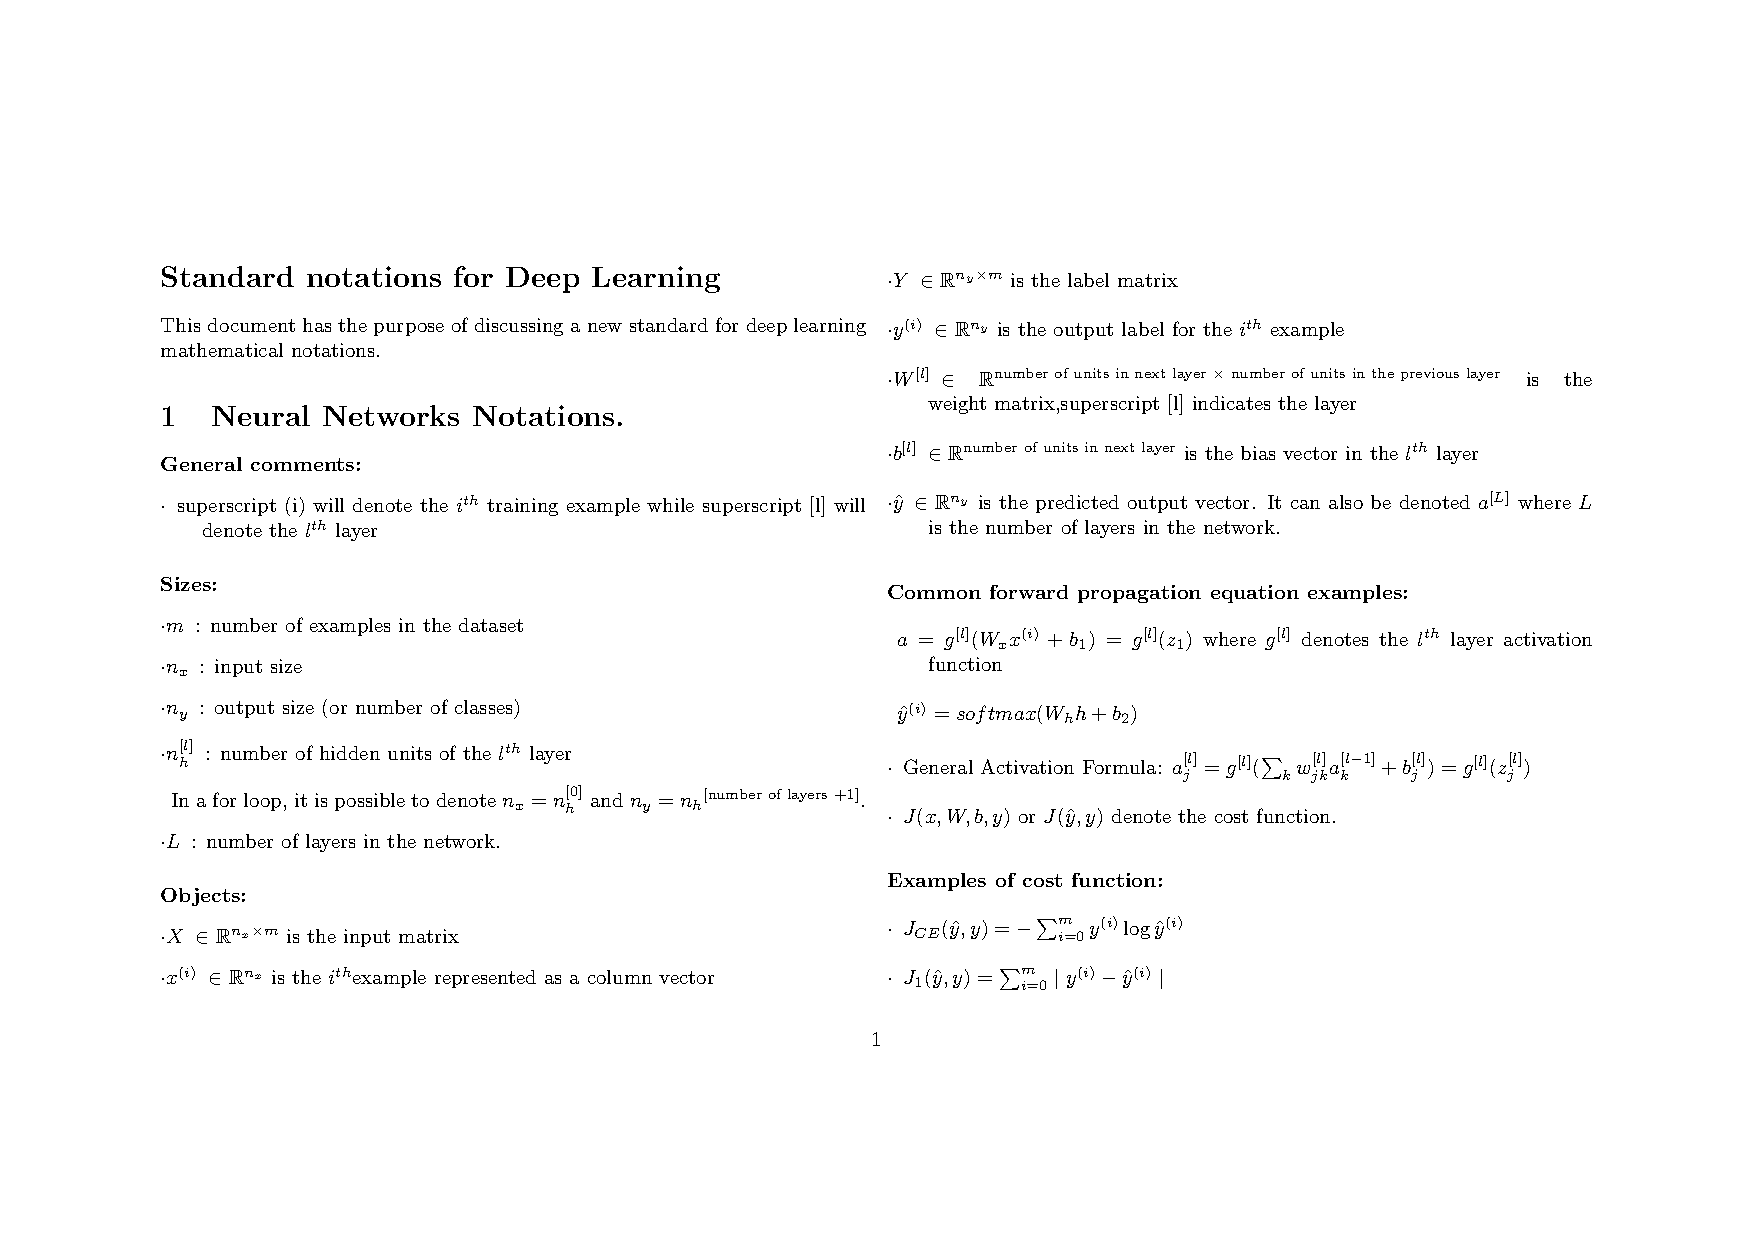
\includepdf[pages={1}, landscape=true]{pdf/deep-learning-notation.pdf}


\chapter{Etapas De Treinamento Utilizando a Rede Neural YOLO } \label{apendice:etapas-yolo}
\begin{itemize}
  \item Criar o arquivo ``yolo-obj.cfg'' com o mesmo conteúdo de ``yolov4-custom.cfg'';
  \item Alterar ``yolo-obj.cfg'' para:
  \begin{itemize}
    \item Considerar \textit{batches} com 64 imagens, onde um \textit{batch} representa o número de amostras a serem trabalhadas antes de atualizar os parâmetros do modelo \cite{ref:Brownlee};
    \item Subdividir cada \textit{batch} em 16 imagens (para processamento paralelo em treinamentos utilizando GPUs - Unidade de Processamento Gráfico do inglês \textit{Graphics Processing Unit});
    \item Utilizar um número máximo de \textit{batches} igual ao produto $n_{classes} \cdot 2000$
    \item Alterar o número de passos de acordo com o número máximo de \textit{batches};
    \item Alterar a quantidade de filtros considerando a fórmula $(n_{classes} + 5) \cdot 3$.
  \end{itemize}
  \item Criar o arquivo ``obj.names'' com os nomes das classes utilizadas, com cada nome em uma linha nova;
  \item Alterar no arquivo ``obj.data'' o número de classes utilizadas;
  \item Colocar as imagens de treinamento e teste no diretório ``obj'' que se encontra dentro de ``data'';
  \item Criar um arquivo de texto com a extensão ``.txt'' para cada uma das imagens do \textit{dataset} no mesmo diretório em que elas estão contendo os objetos e suas respectivas coordenadas, seguindo o padrão  $<objectclass> <x_{center}> <y_{center}> <width> <height>$ de forma que cada linha represente um objeto, onde
  \begin{itemize}
    \item $<objectclass>$ indica a classe do objeto de acordo com a ordem definida no arquivo ``obj.names'' com valores dentro do intervalo $[0, n_{classes} - 1]$;
    \item $<x_{center}> <y_{center}>$ são as coordenadas centrais da localização da caixa delimitadora do objeto, valores em ponto flutuante dentro do intervalo $[0.0, 1.0]$, normalizados de acordo com o tamanho da imagem utilizada.
    \item $<width> <height>$ são a largura e a altura, respectivamente, da caixa delimitadora do objeto, valores em ponto flutuante dentro do intervalo $[0.0, 1.0]$, normalizados de acordo com o tamanho da imagem utilizada.
  \end{itemize}
  \item Criar os arquivos de texto ``train.txt'' e ``test.txt'' que contém o nome das imagens utilizadas no treinamento e teste, respectivamente, onde para cada imagem utiliza-se uma nova linha;
  \item Fazer o \textit{download} de pesos pré-treinados, com intuído de acelerar o treinamento;
  \item Iniciar o treinamento.
\end{itemize}


\chapter{Placas de Circuito Impresso Utilizadas para o Conjunto de Dados HRIPCB} \label{apendice:hripcb-pcbs}

\begin{figure}[!h] %H
  \centering
  \caption{PCI Número 01 do conjunto de dados HRIPCB.}
  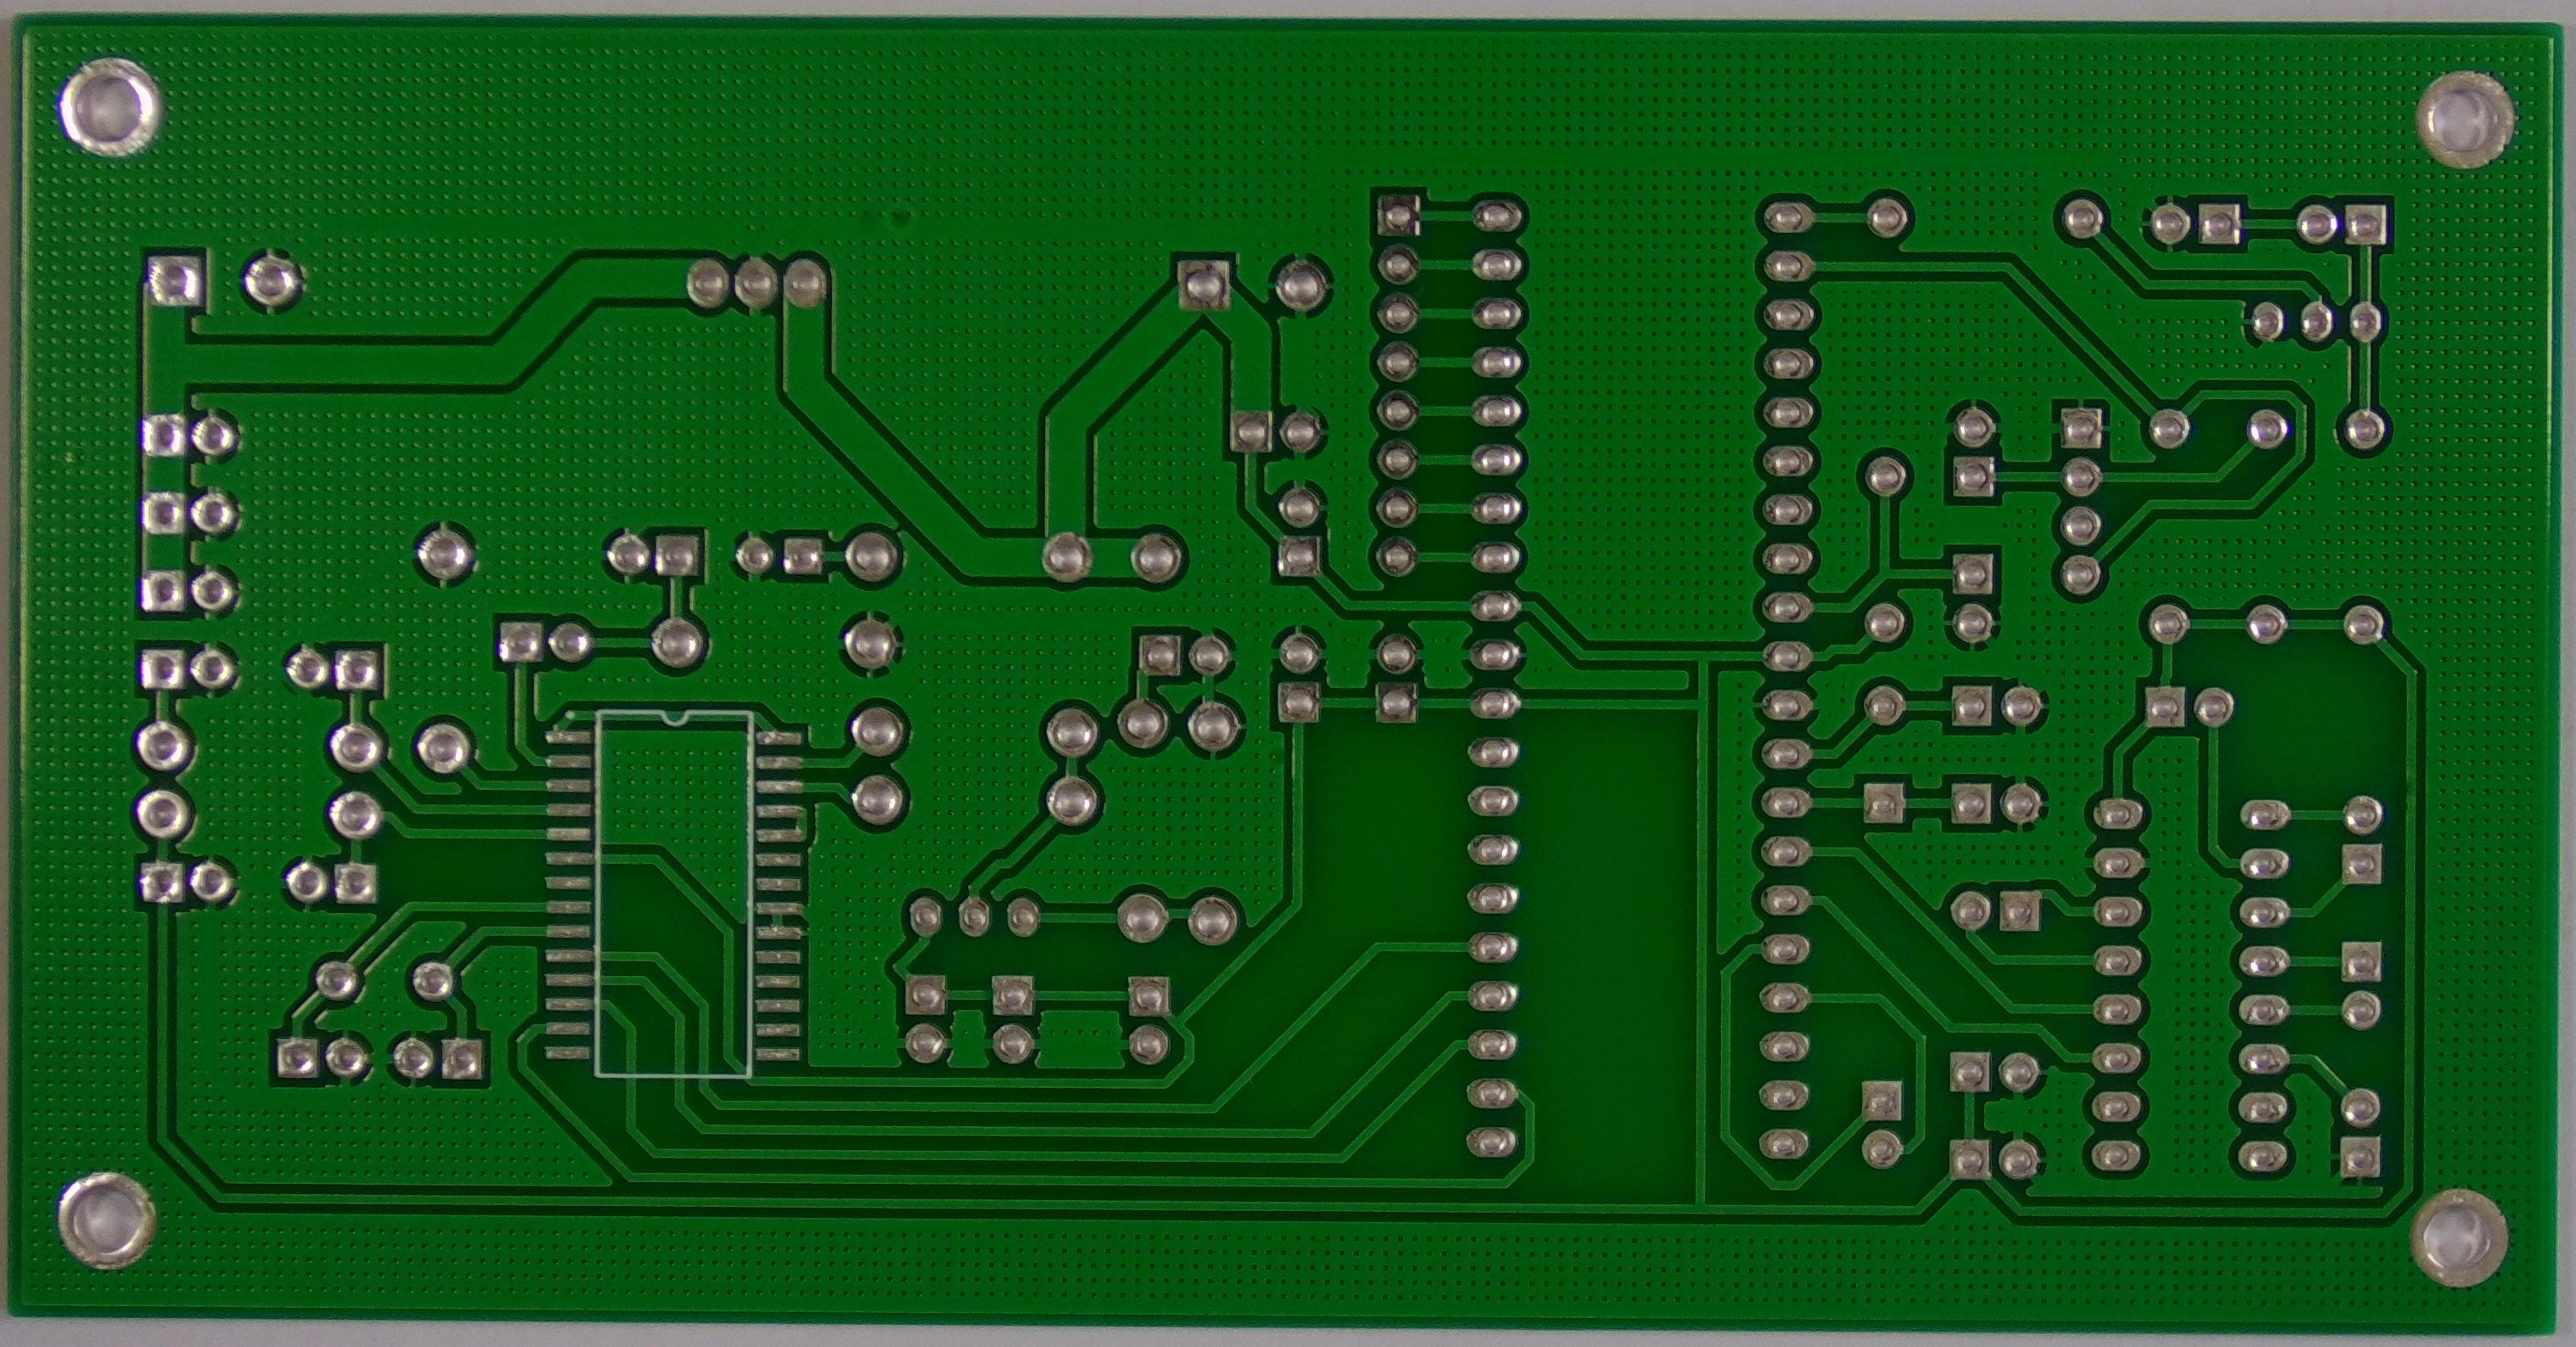
\includegraphics[scale=0.11]{img/pcbs/01.JPG}
  \label{fig:ap-pcbs-1}
  \indentedfont[15.2cm]{\citeonline{ref:Huang-et-al}}
\end{figure}

\begin{figure}[!h] %H
  \centering
  \caption{PCI Número 04 do conjunto de dados HRIPCB.}
  \includegraphics[scale=0.11]{img/pcbs/04.JPG}
  \label{fig:ap-pcbs-4}
  \indentedfont[15.2cm]{\citeonline{ref:Huang-et-al}}
\end{figure}

\begin{figure}[!h] %H
  \centering
  \caption{PCI Número 05 do conjunto de dados HRIPCB.}
  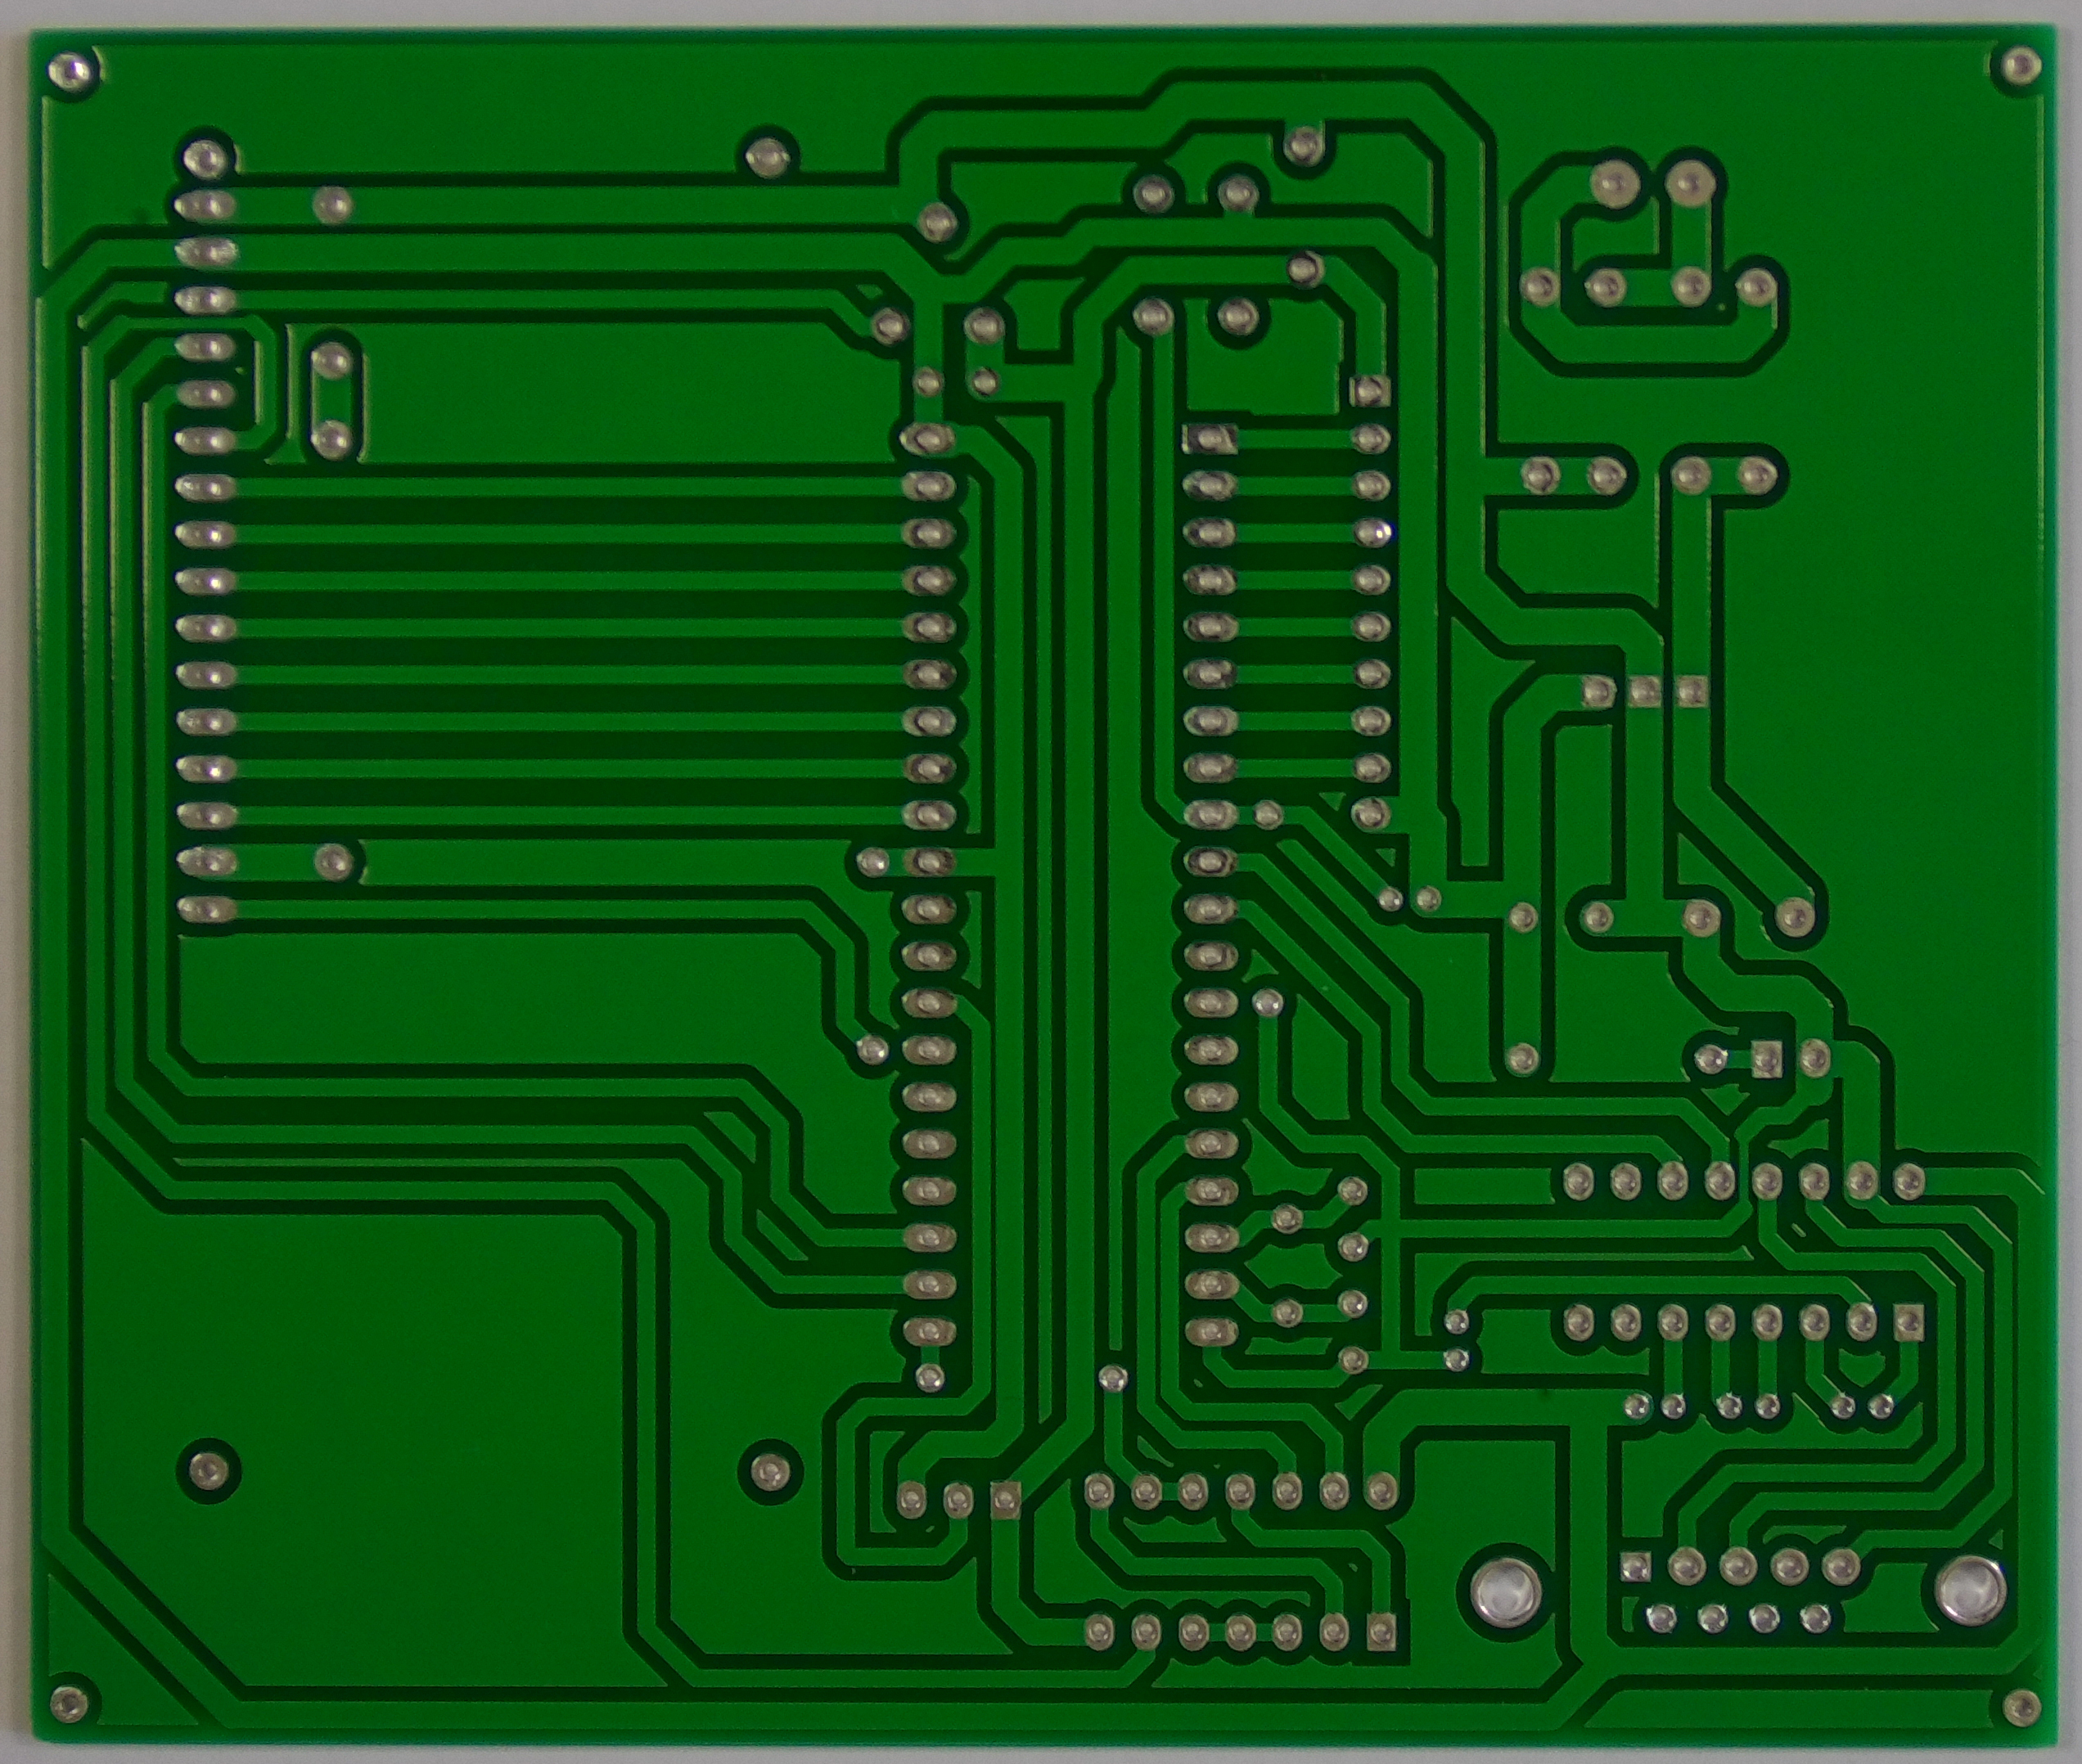
\includegraphics[scale=0.13]{img/pcbs/05.JPG}
  \label{fig:ap-pcbs-5}
  \indentedfont[15.2cm]{\citeonline{ref:Huang-et-al}}
\end{figure}

\begin{figure}[!h] %H
  \centering
  \caption{PCI Número 06 do conjunto de dados HRIPCB.}
  \includegraphics[scale=0.13]{img/pcbs/06.JPG}
  \label{fig:ap-pcbs-6}
  \indentedfont[15.2cm]{\citeonline{ref:Huang-et-al}}
\end{figure}

\begin{figure}[!h] %H
  \centering
  \caption{PCI Número 07 do conjunto de dados HRIPCB.}
  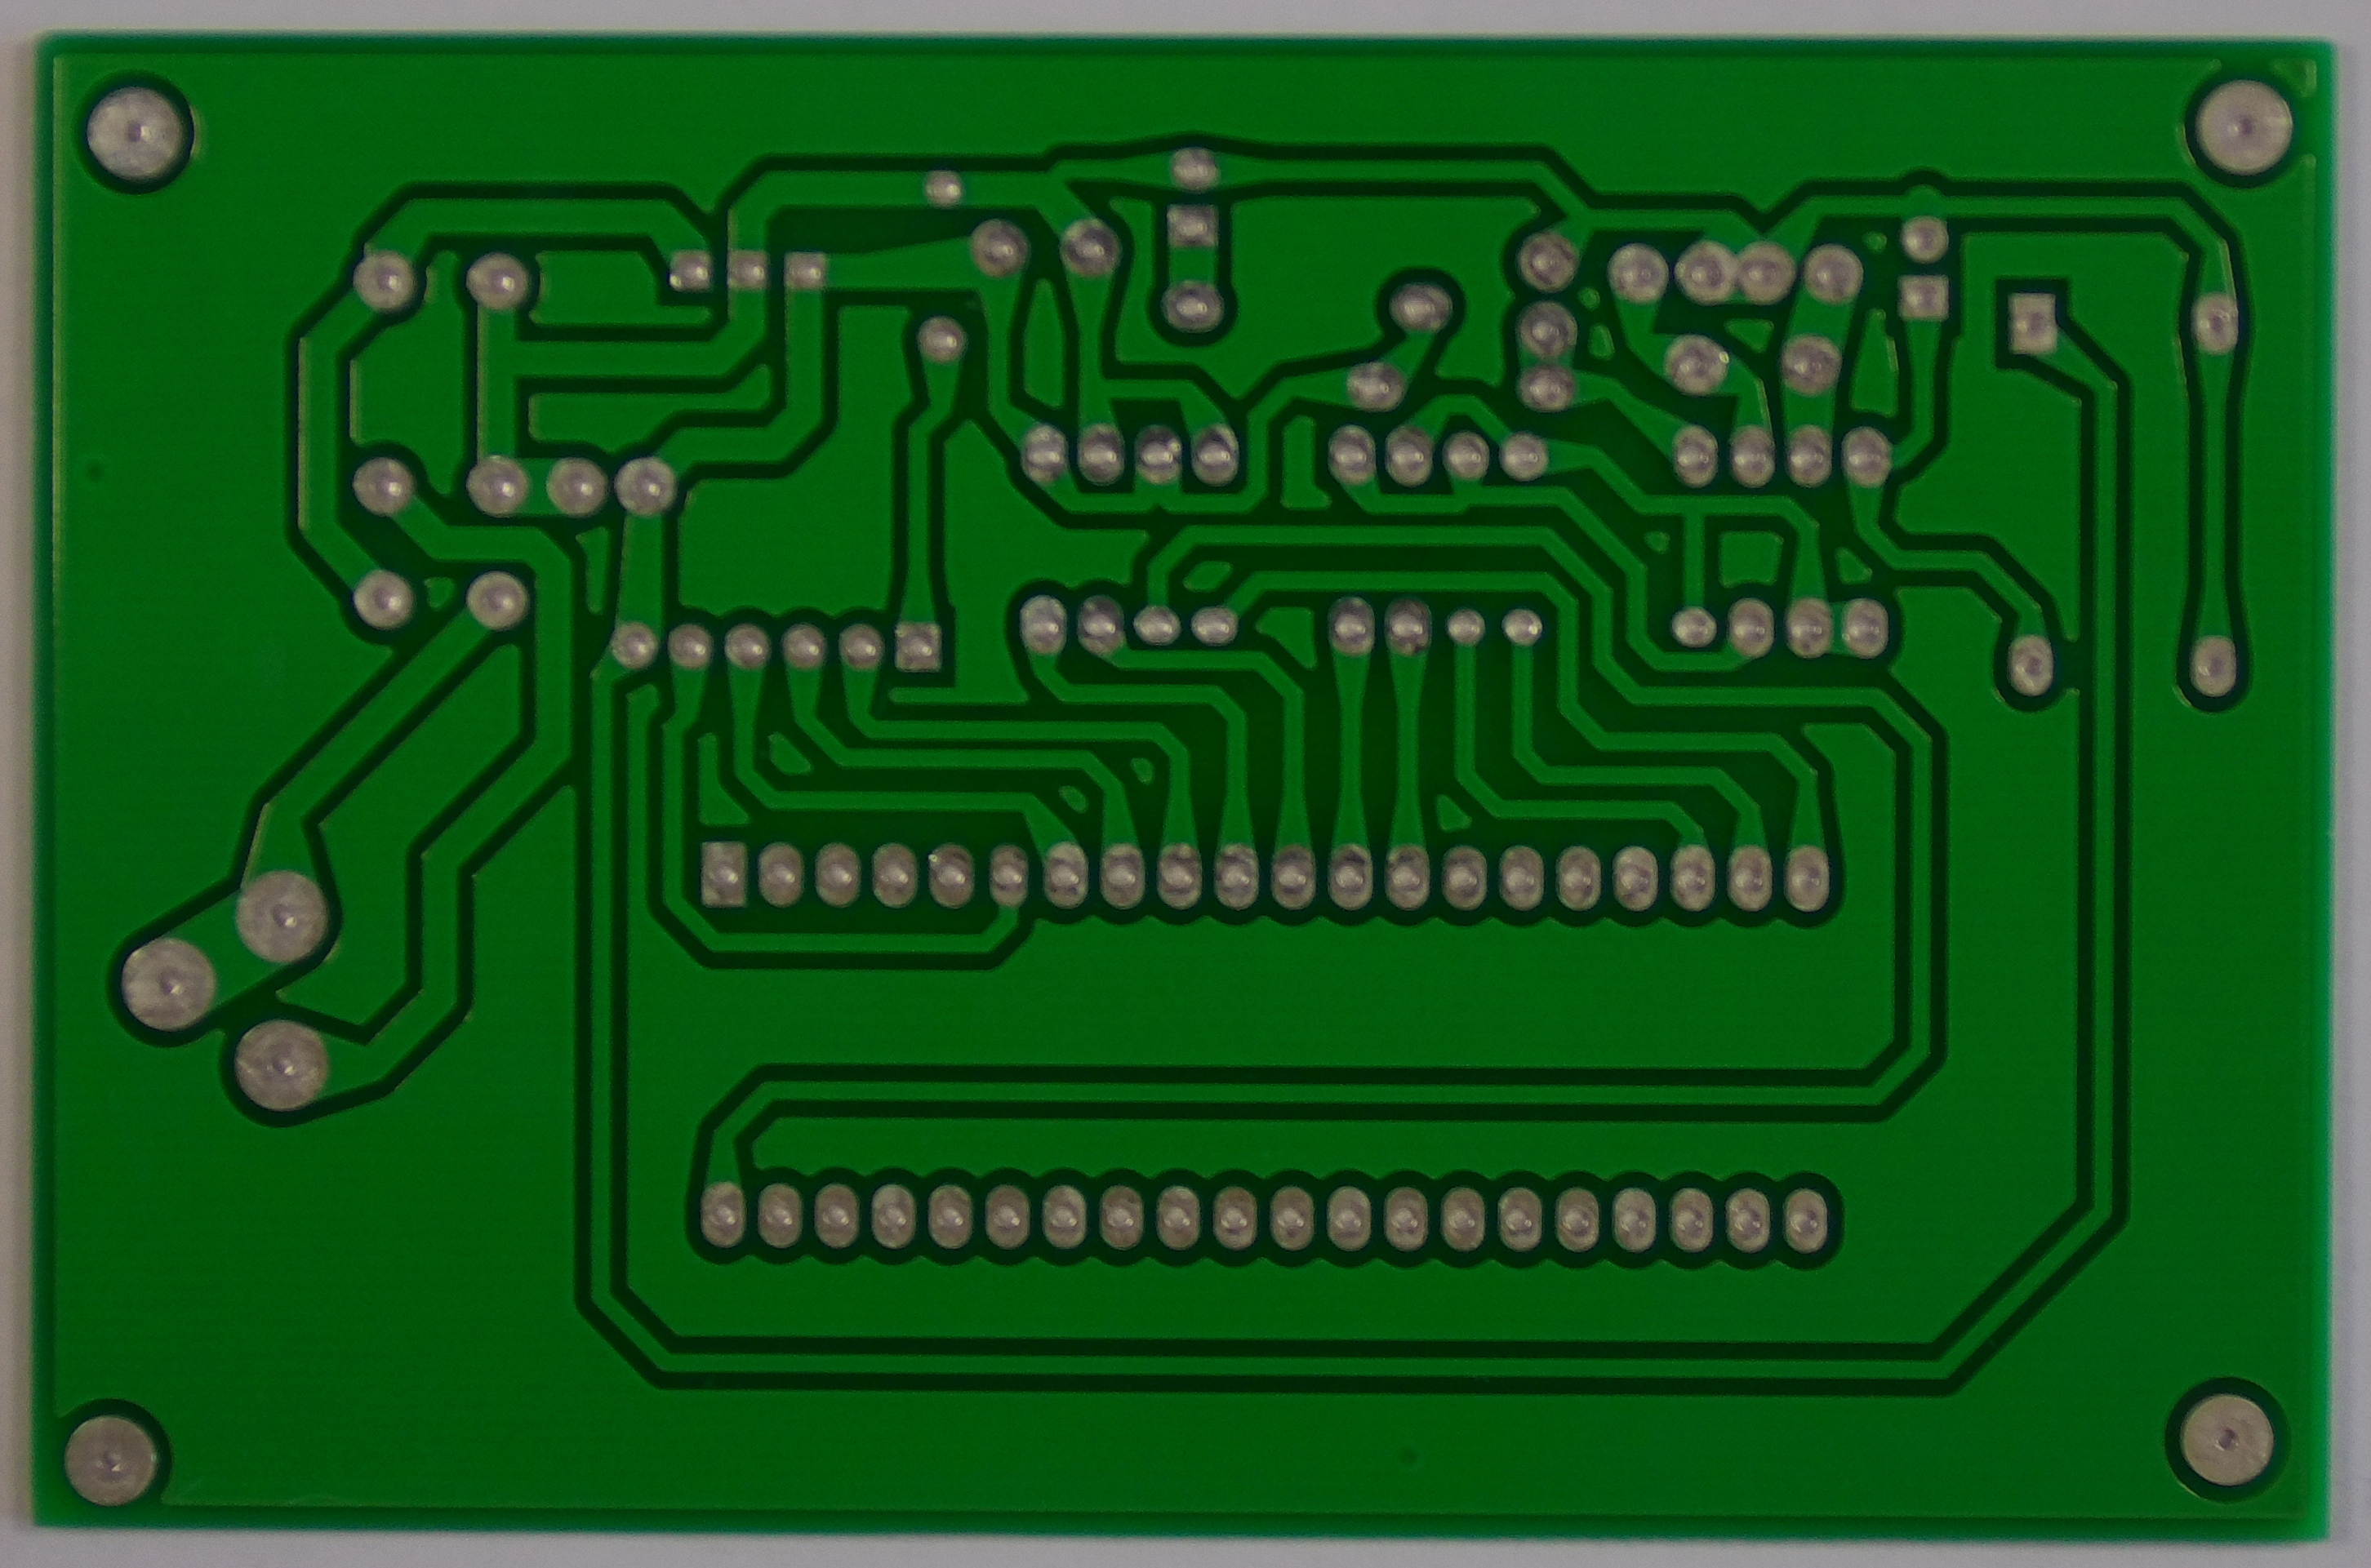
\includegraphics[scale=0.13]{img/pcbs/07.JPG}
  \label{fig:ap-pcbs-7}
  \indentedfont[15.2cm]{\citeonline{ref:Huang-et-al}}
\end{figure}

\begin{figure}[!h] %H
  \centering
  \caption{PCI Número 08 do conjunto de dados HRIPCB.}
  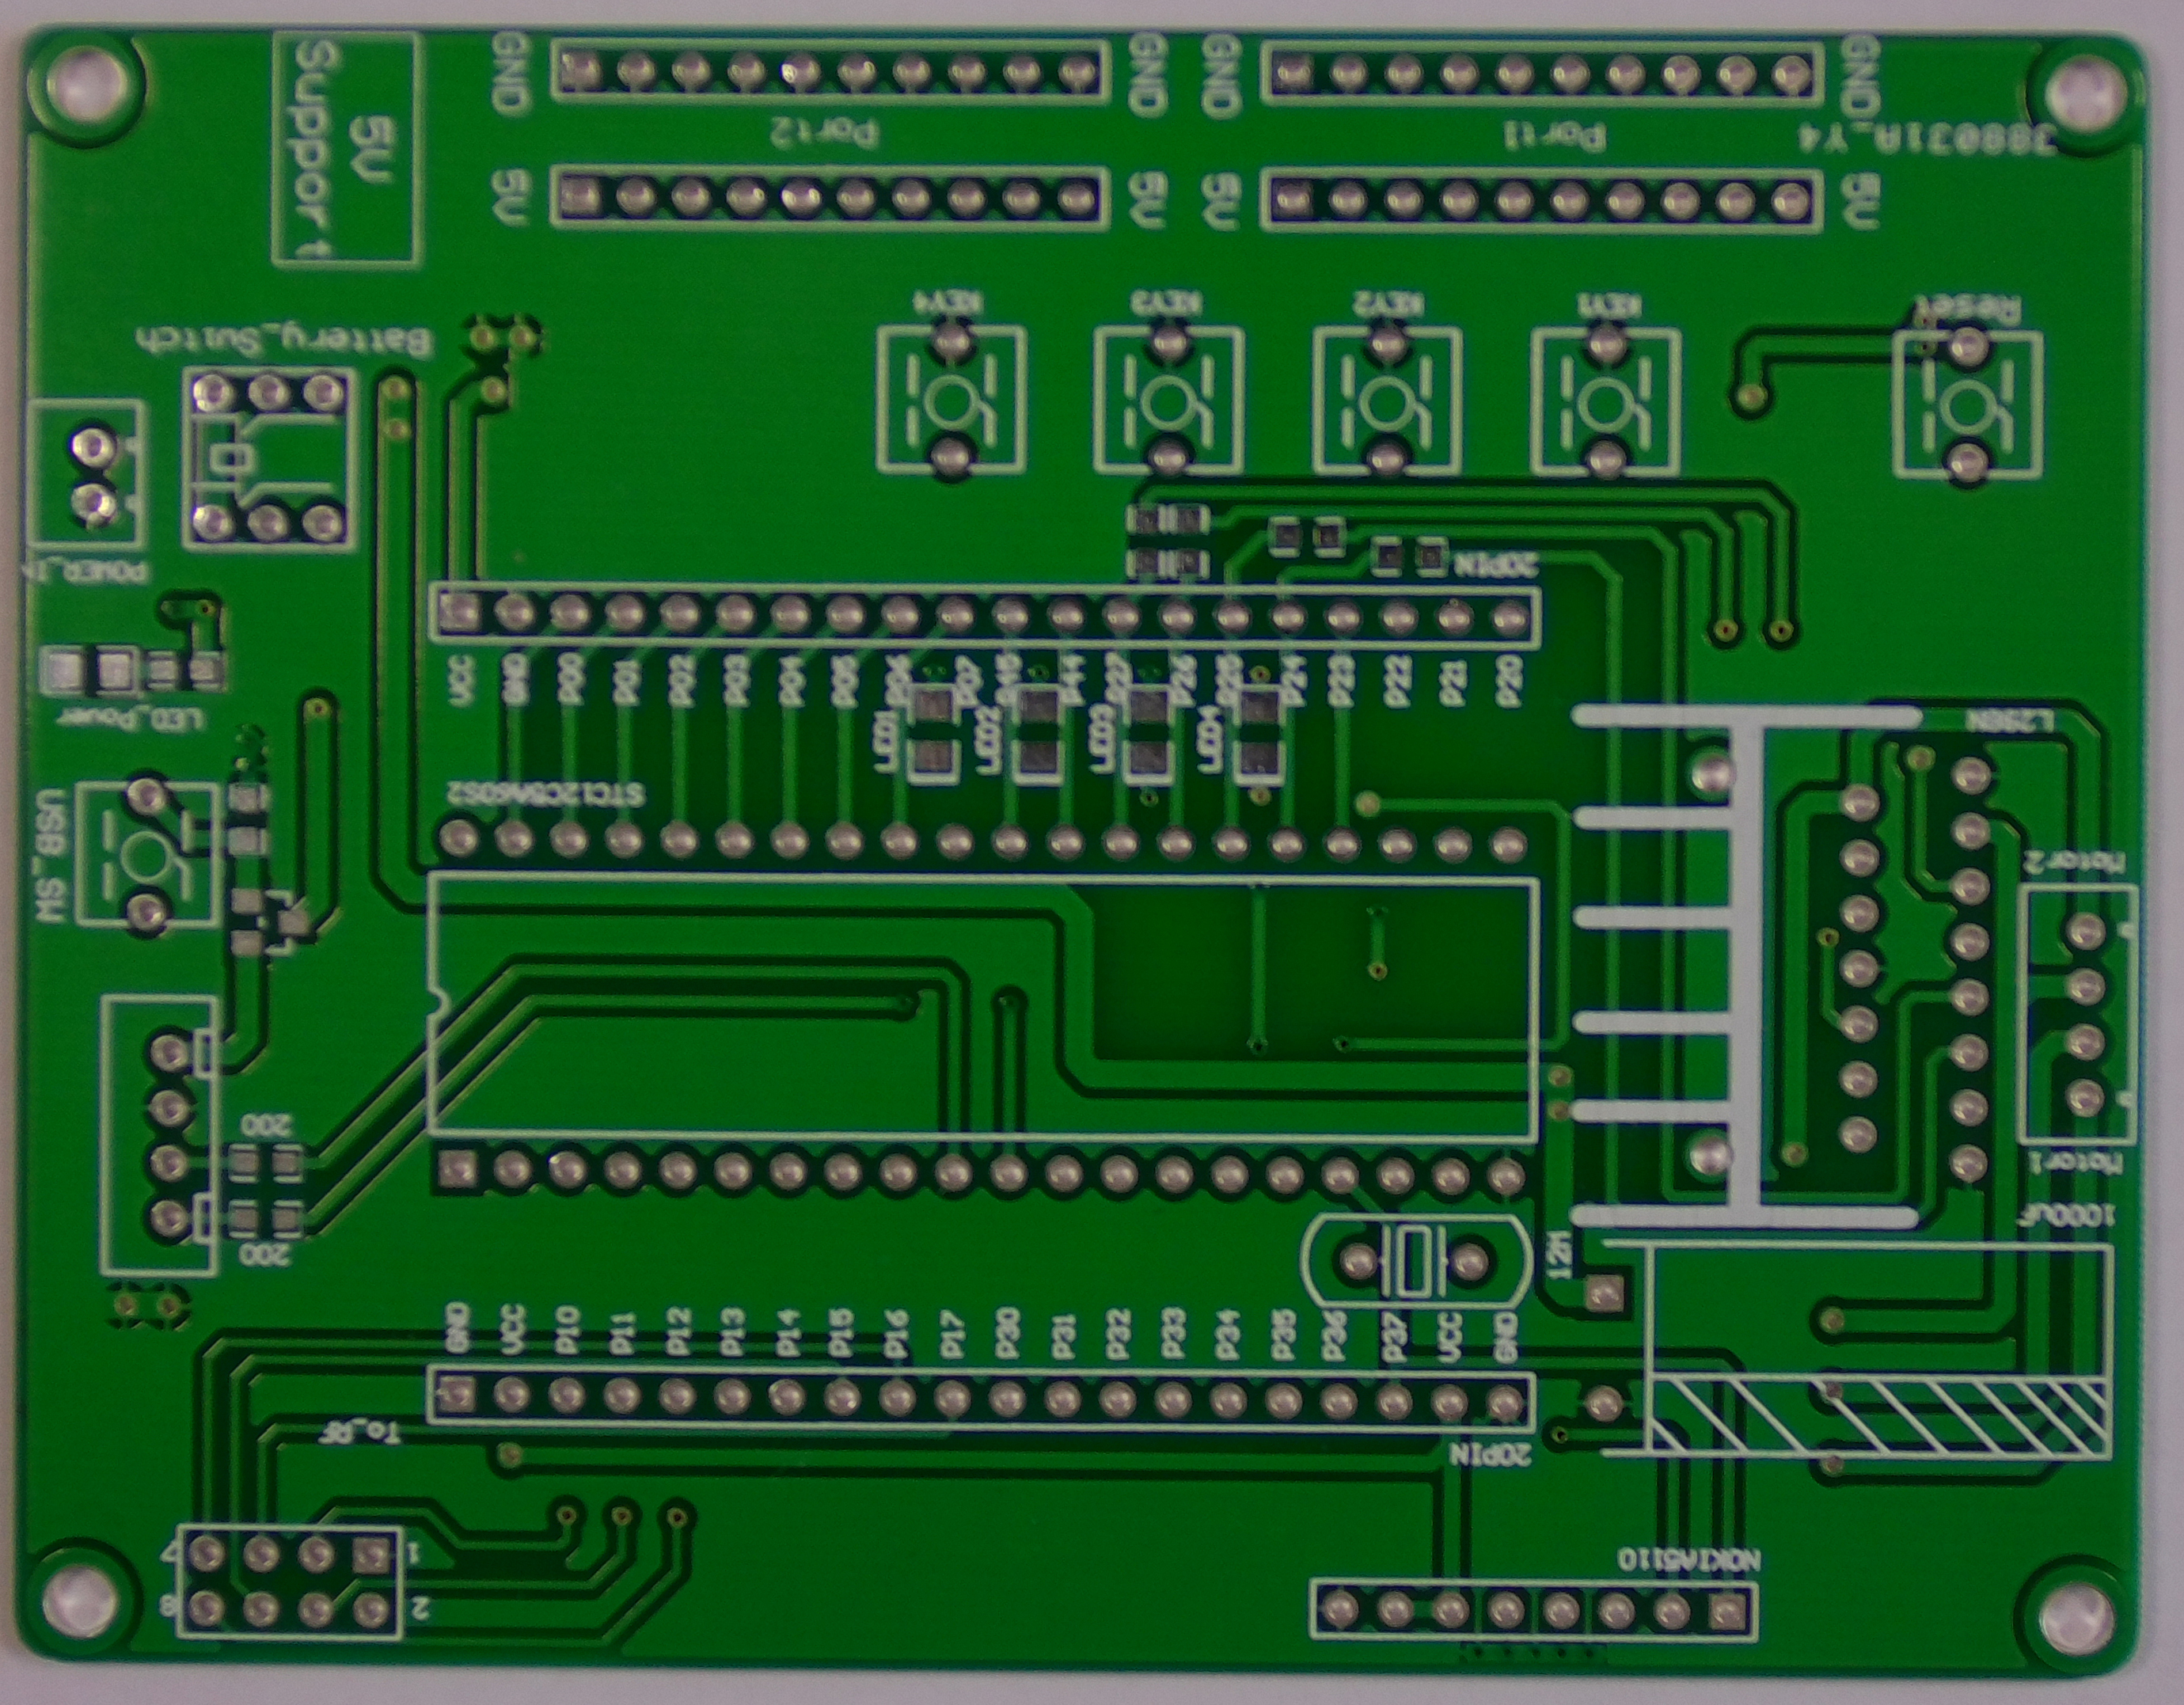
\includegraphics[scale=0.13]{img/pcbs/08.JPG}
  \label{fig:ap-pcbs-8}
  \indentedfont[15.2cm]{\citeonline{ref:Huang-et-al}}
\end{figure}

\begin{figure}[!h] %H
  \centering
  \caption{PCI Número 09 do conjunto de dados HRIPCB.}
  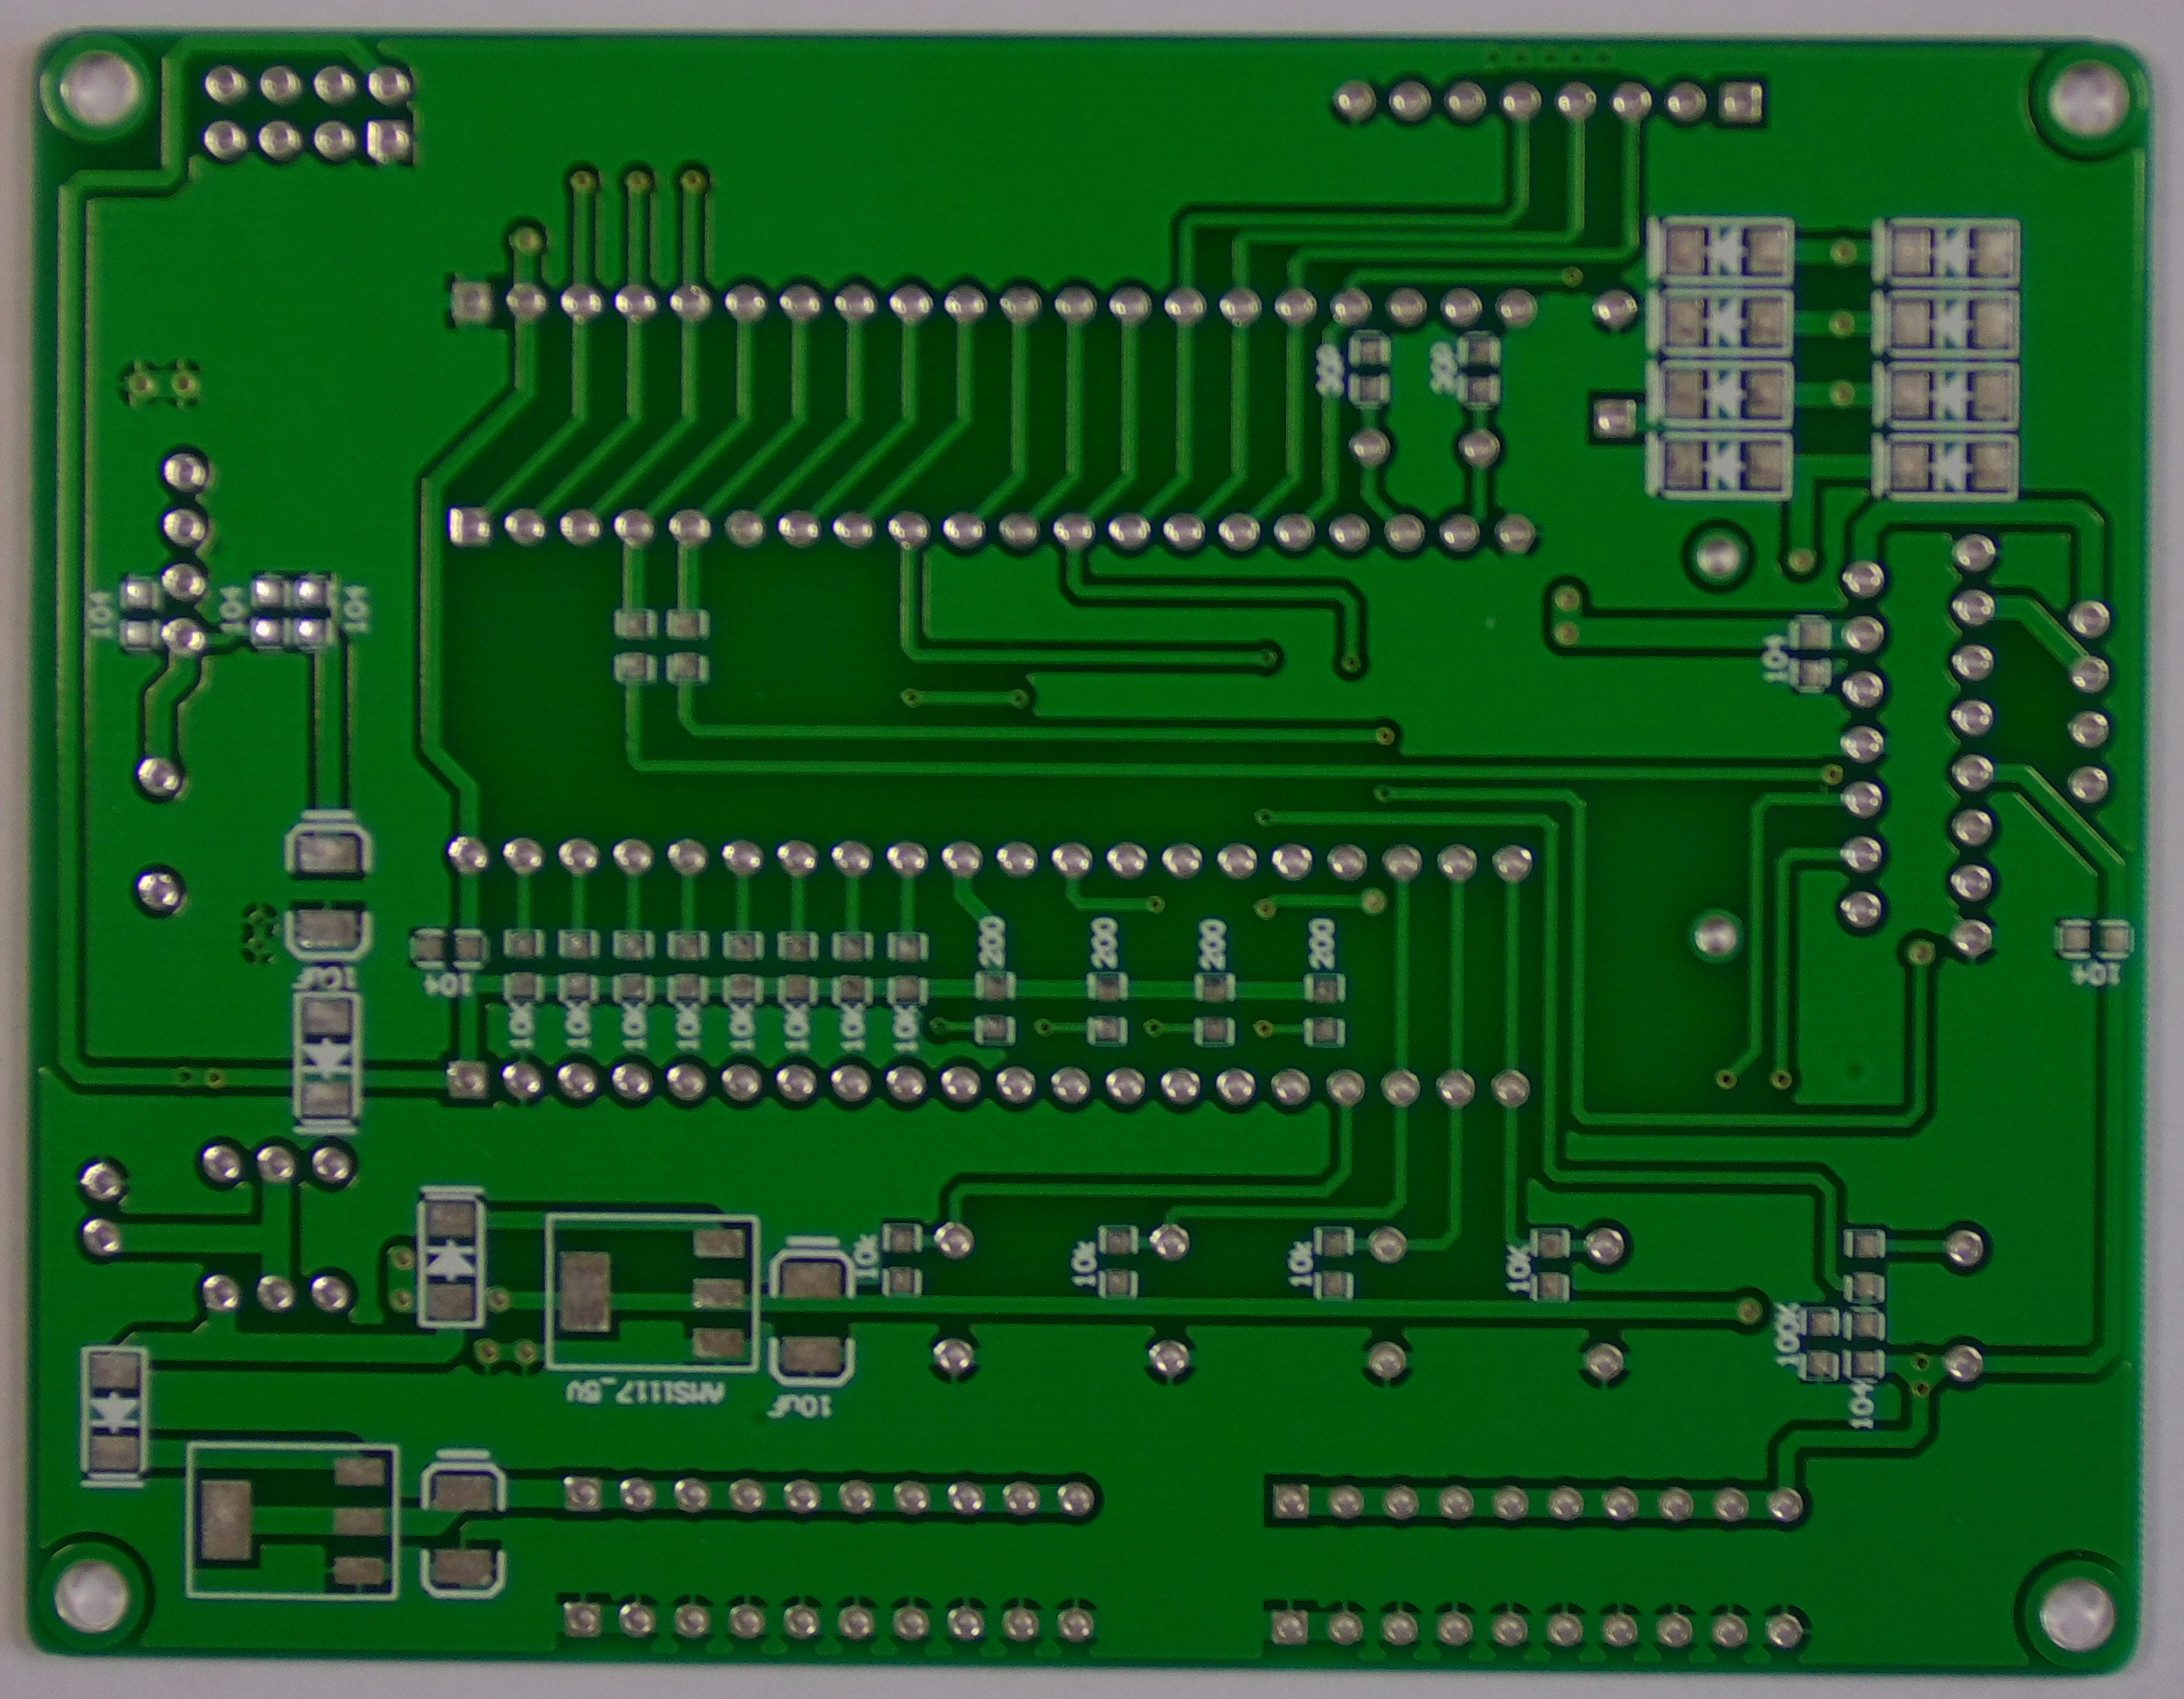
\includegraphics[scale=0.13]{img/pcbs/09.JPG}
  \label{fig:ap-pcbs-9}
  \indentedfont[15.2cm]{\citeonline{ref:Huang-et-al}}
\end{figure}

\begin{figure}[!h] %H
  \centering
  \caption{PCI Número 10 do conjunto de dados HRIPCB.}
  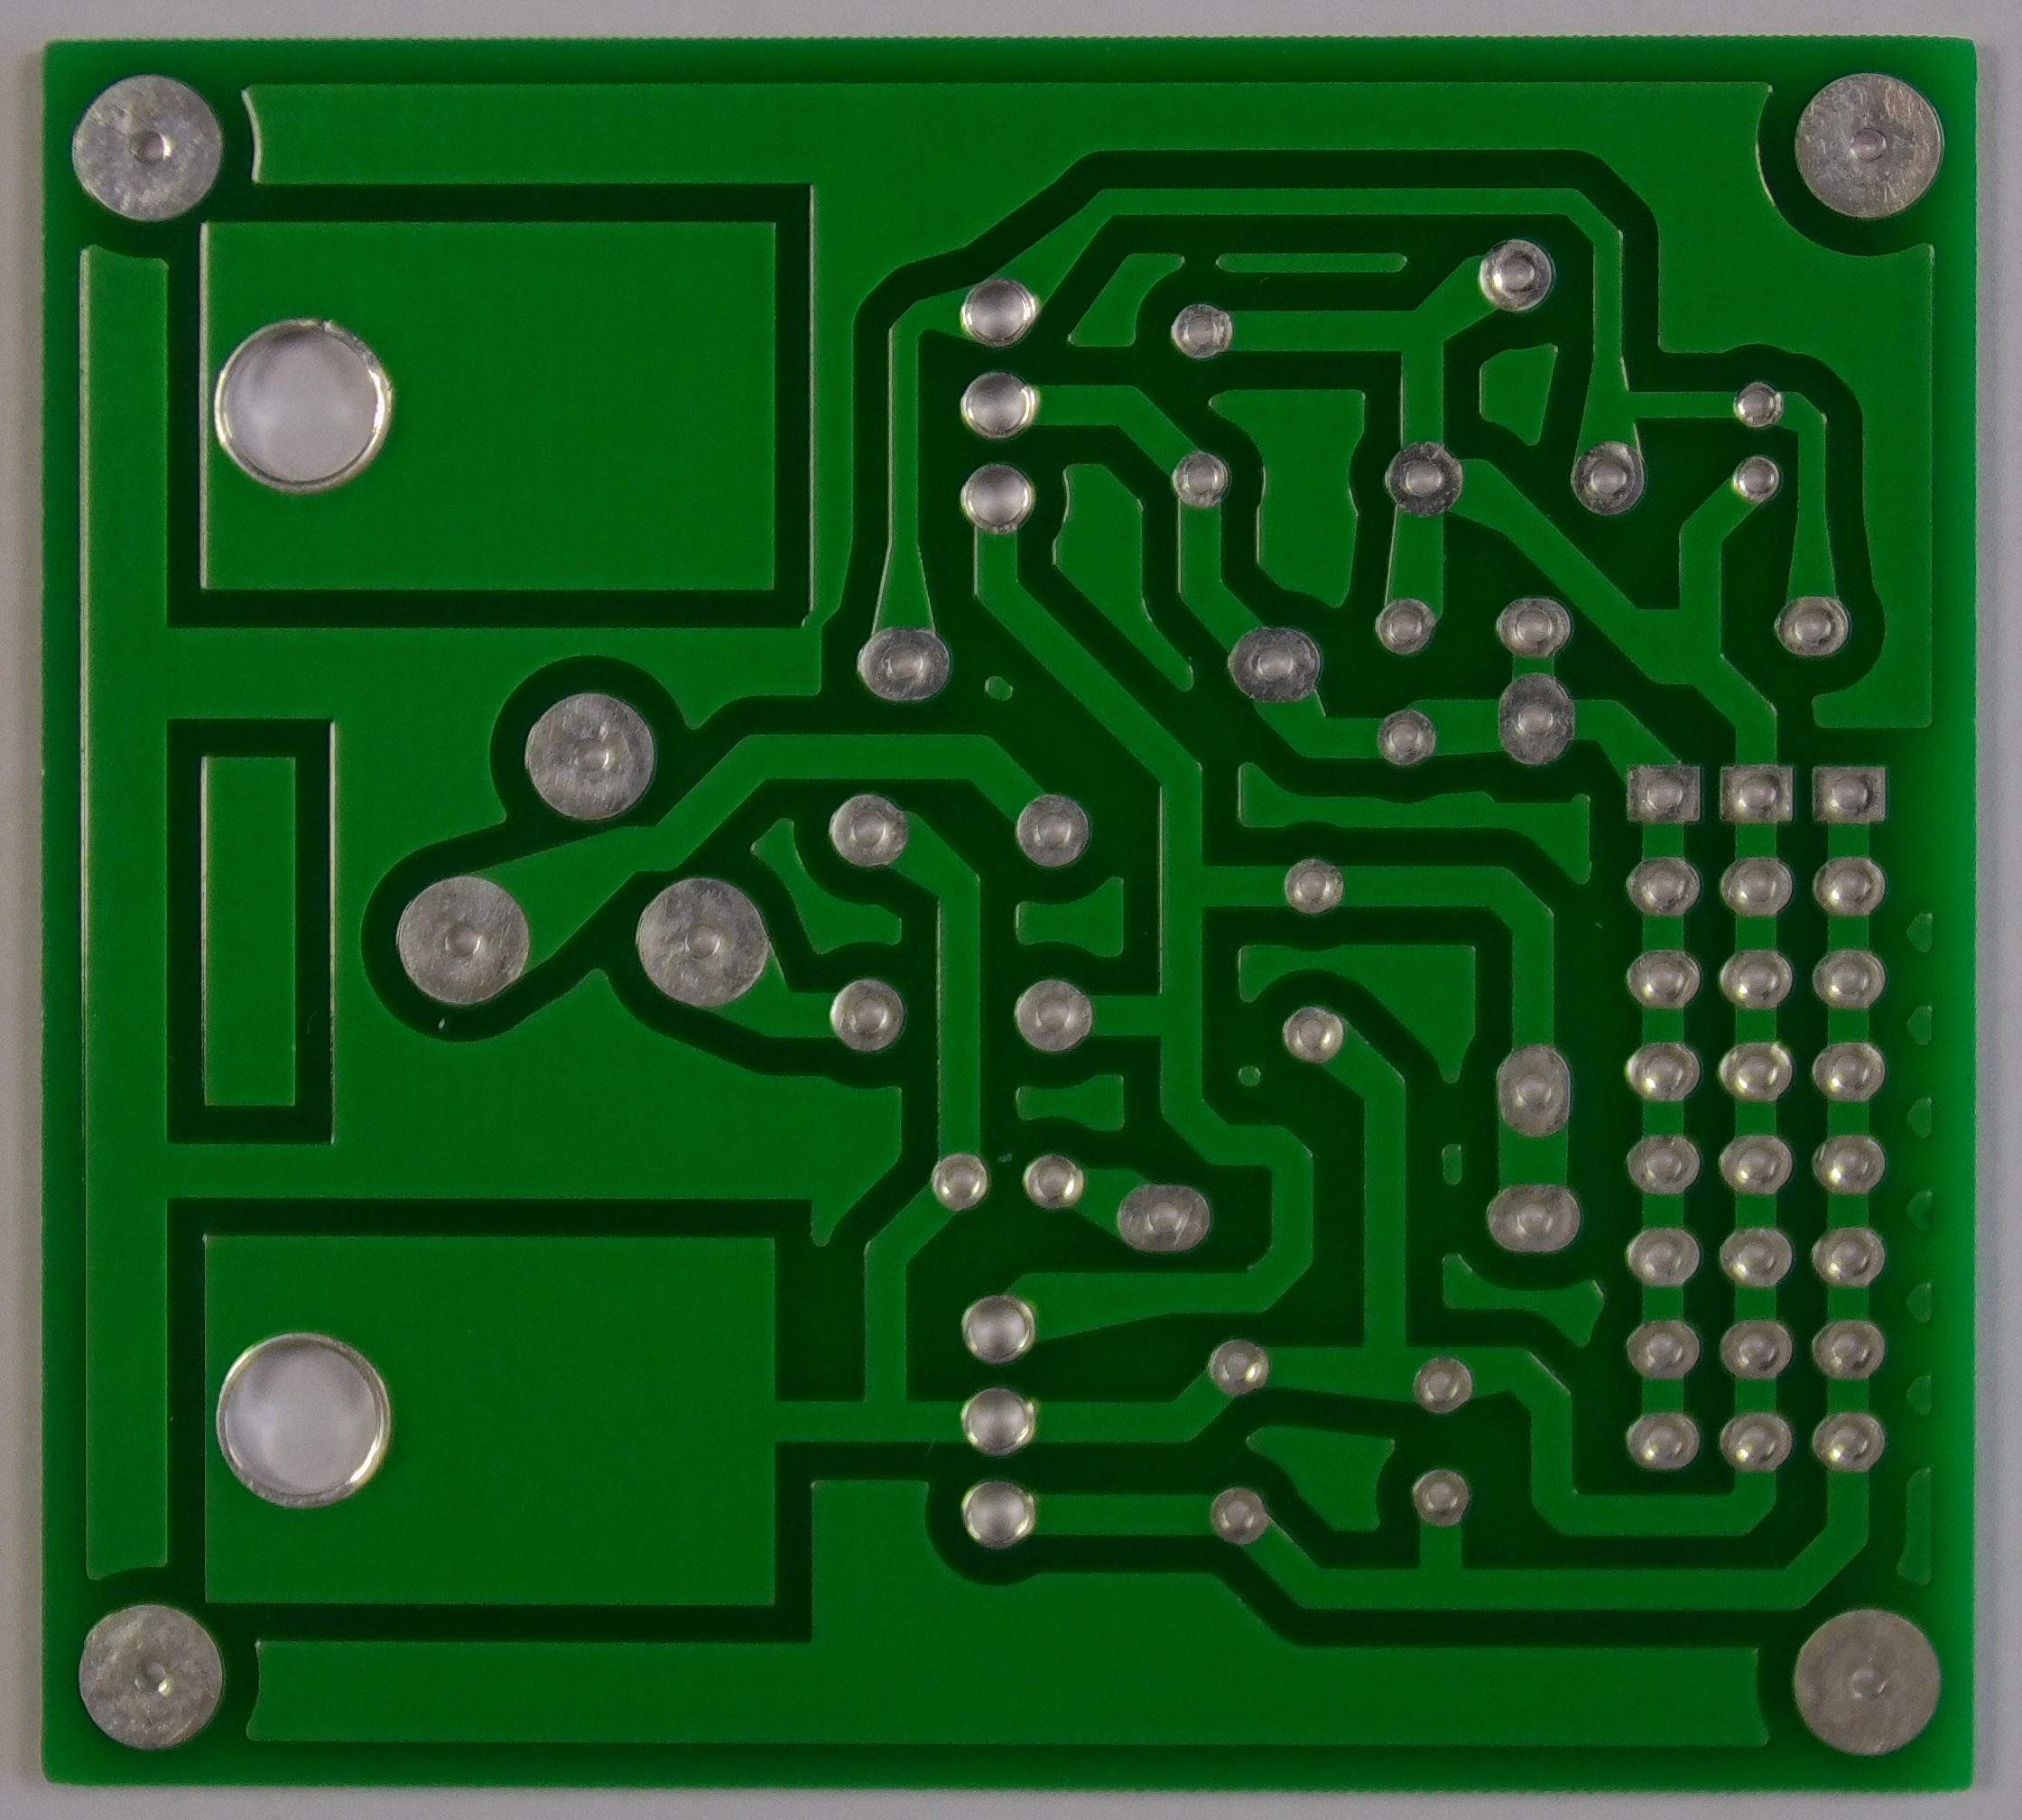
\includegraphics[scale=0.13]{img/pcbs/10.JPG}
  \label{fig:ap-pcbs-10}
  \indentedfont[15.2cm]{\citeonline{ref:Huang-et-al}}
\end{figure}

\begin{figure}[!h] %H
  \centering
  \caption{PCI Número 11 do conjunto de dados HRIPCB.}
  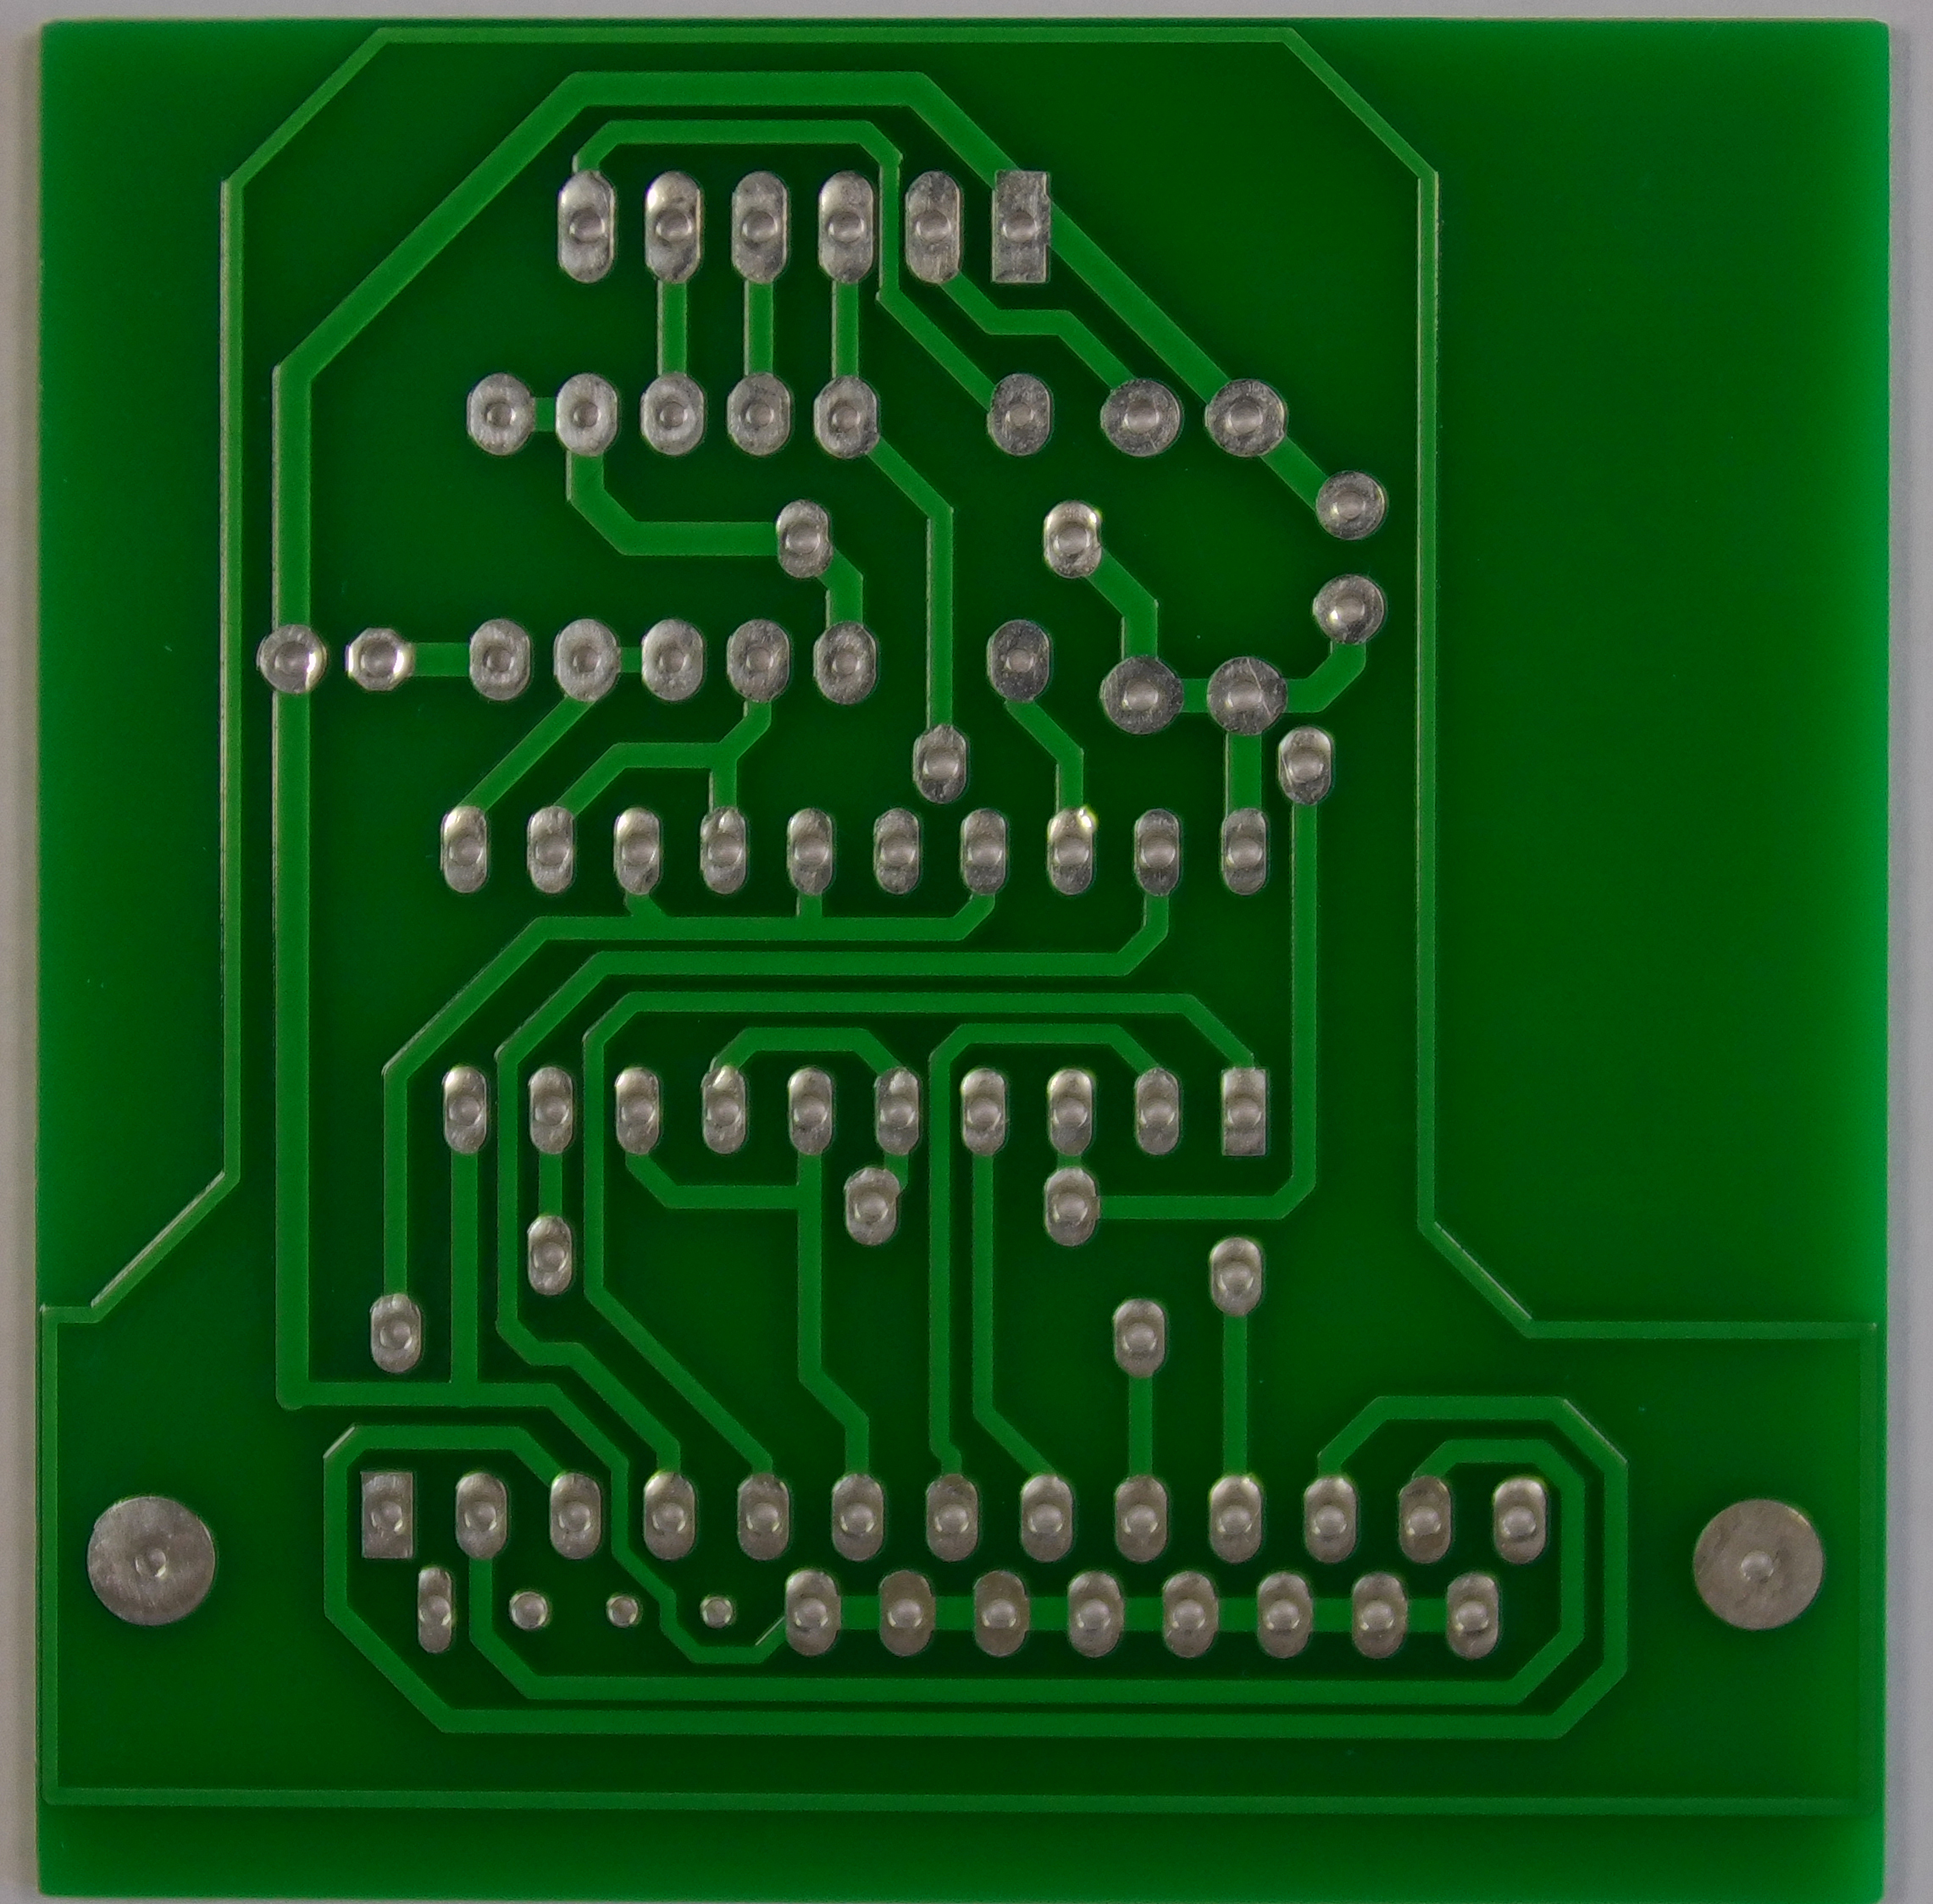
\includegraphics[scale=0.13]{img/pcbs/11.JPG}
  \label{fig:ap-pcbs-11}
  \indentedfont[15.2cm]{\citeonline{ref:Huang-et-al}}
\end{figure}

\begin{figure}[!h] %H
  \centering
  \caption{PCI Número 12 do conjunto de dados HRIPCB.}
  \includegraphics[scale=0.11]{img/pcbs/12.JPG}
  \label{fig:ap-pcbs-12}
  \indentedfont[15.2cm]{\citeonline{ref:Huang-et-al}}
\end{figure}


\chapter{Exemplo de Arquivo de Anotação do Conjunto de Dados HRIPCB em XML} \label{apendice:hripcb-xml}
\lstinputlisting[caption=Arquivo de Anotação do \textit{Dataset} HRIPCB., label=lst:hripcb, firstnumber=1, language=XML]{cod/anotacoes-HRIPCB.xml}

\chapter{\textit{Script} Utilizado na Conversão dos Arquivos de Anotação} \label{apendice:conversao}
\lstinputlisting[caption=\textit{Script para conversão de arquivos de anotação de xml pata txt.}, label=lst:conversao, firstnumber=1, language=Python]{cod/HRIPCB_yolo_dataset_config.py}

\chapter{\textit{Script} Utilizado na Divisão do \textit{Dataset} para Treinamento da Rede Neural} \label{apendice:divisao}
\lstinputlisting[caption=\textit{Script} para divisão do \textit{dataset}., label=lst:conversao, firstnumber=1, language=Python]{cod/dataset_split.py}

\chapter{Código Utilizado para o Treinamento da Rede Neural no Ambiente Google Colab} \label{apendice:treinamento}
\lstinputlisting[caption=Comandos executados no ambiente Google Colab para o treinamento da Rede Neural., label=lst:treinamento, firstnumber=1, language=Python]{cod/treinamento.py}

\chapter{Configurações Para a Execução da Interface de Aplicação De Detecção de Defeitos em Placas de Circuito Impresso} \label{apendice:conf-api}

\lstinputlisting[caption=Compilando o Darknet, label=lst:conf-api, firstnumber=1]{cod/api-config.md}

\lstinputlisting[caption=Executando a Interface de Aplicação, label=lst:conf-api, firstnumber=1]{cod/api-config-2.md}
%\markdownInput{cod/README.md}



%\chapter{Arquivos de Configuração para o Treinamento com YOLOv4 utilizando Darknet} \label{apendice:treinamento-cfg}
%\lstinputlisting[label=lst:treinamento, firstnumber=1]{cod/yolov4_custom.cfg}

%\end{apendicesenv}

% ----------------------------------------------------------
% Anexos
% ----------------------------------------------------------
%\begin{anexosenv}
%    \partanexos
%    \chapter{Meu primeiro assunto de anexo}


\chapter{Segundo assunto que pesquisei}

%\end{anexosenv}

%---------------------------------------------------------------------
% INDICE REMISSIVO
%---------------------------------------------------------------------
%\phantompart
%\printindex
%---------------------------------------------------------------------

\end{document}
